\chapter{离散信道的容量}
\label{chap:discrete-channel-capacity}

通过一条线路发送二进制符号，每个符号以$10\%$的概率被翻转。把每个比特连发三遍、接收端取多数，错误率可以从$0.1$降到$0.028$，代价是每次使用线路只送出$1/3$比特。连发更多遍，错误还会继续下降，但每次使用承载的信息也趋于零。是否存在一种办法，既让错误任意小，又让每次使用平均送出一个固定的正比特数？如果存在，这个比特数最多能有多大？

答案是一个由信道本身决定的数，称为容量。对上面的线路，它约为$0.531$比特每次使用：低于这个速率，适当设计的长码可以使错误概率趋于零；高于这个速率，任何码的错误概率都不能趋于零。直观地说，容量回答“每次传输最多能区分多少种消息”：一次使用若能可靠地区分$2^{C}$种情形，$n$次使用就能区分约$2^{nC}$条消息。

本章研究输入、输出都取有限个值、各次使用互不影响的信道。先用条件概率矩阵描述信道，再规定块码、码率与错误概率的口径；然后把容量写成单次互信息在输入分布上的最大值，并证明它恰好是可靠传输速率的极限。随后计算二元对称信道与二元擦除信道的容量，研究输入有成本时的容量，最后给出数值计算容量的Blahut–Arimoto迭代。

全章以2为底取对数，熵、互信息与KL散度都以比特（bit）计，容量与码率的单位是比特每次信道使用。所用的熵、条件熵、互信息、KL散度、数据处理不等式与Fano不等式取自第~\ref{chap:information-measures}章，那里用自然对数，换成以2为底只把每个量乘以常数$1/\ln2$，不改变任何不等式。条件分布的写法取自第~\ref{chap:conditional-distributions}章，大数律取自第~\ref{chap:laws-of-large-numbers}章。

\section{离散无记忆信道}
\label{sec:dcc-dmc}

发送端送出一个符号，接收端收到另一个符号，两者之间的关系不确定但有规律。数学上，这种规律就是给定输入时输出的条件分布。先看三个二元输入的例子，它们在全章反复出现。

\paragraph{三个例子}
\term{二元对称信道}（binary symmetric channel，BSC）的输入、输出都是$\{0,1\}$，每个符号独立地以概率$p$被翻转，以概率$1-p$原样到达。\term{二元擦除信道}（binary erasure channel，BEC）的输出多一个符号$\mathrm{e}$：每个符号以概率$\varepsilon$被“擦掉”，接收端看到$\mathrm{e}$，知道这里丢了东西；以概率$1-\varepsilon$原样到达，不会出现翻转。\term{Z信道}（Z-channel）只有一个方向出错：输入$0$总是正确到达，输入$1$以概率$\tfrac12$变成$0$。图~\ref{fig:dcc-channel-diagrams}画出三者的转移图，每个输入发出的箭头上的概率之和为$1$。

\begin{BookInlineFigure}
 \centering
 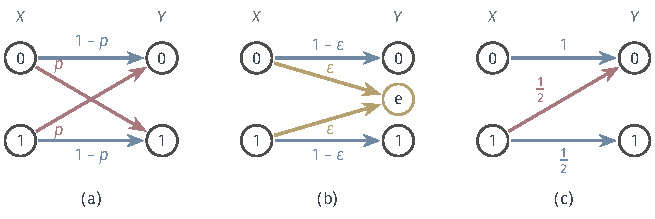
\includegraphics[width=110.9mm]{figures/07-probability/06-channel-coding/tikz/dcc-channel-diagrams/figure.pdf}
 \caption{三个二元输入信道的转移图，箭头上的数是条件概率$W(y\mid x)$。(a) 二元对称信道，红色箭头表示翻转；(b) 二元擦除信道，黄色箭头通向接收端可见的擦除符号$\mathrm{e}$；(c) 本章所用的Z信道，输入$1$以概率$\tfrac12$变成$0$。}
 \label{fig:dcc-channel-diagrams}
\end{BookInlineFigure}

把这些例子的共同结构抽出来：有限的输入字母表、有限的输出字母表，以及每个输入对应的一张输出概率表。

\begin{definition}[离散信道]
\label{def:dcc-channel}
设$\mathcal{X}$、$\mathcal{Y}$是有限集。一个从$\mathcal{X}$到$\mathcal{Y}$的离散信道由一族非负数$W(y\mid x)$给出（$x\in\mathcal{X}$，$y\in\mathcal{Y}$），满足
\begin{equation}
 \sum_{y\in\mathcal{Y}}W(y\mid x)=1,\qquad x\in\mathcal{X} .
 \label{eq:dcc-channel-rows}
\end{equation}
$W(y\mid x)$是输入为$x$时输出为$y$的概率。把它排成$\lvert\mathcal{X}\rvert\times\lvert\mathcal{Y}\rvert$矩阵$\bm{W}$，第$x$行记为$W_x=W(\cdot\mid x)$，称$\bm{W}$为信道的转移矩阵。
\end{definition}

条件~\eqref{eq:dcc-channel-rows}说每一行都是$\mathcal{Y}$上的概率分布。用第~\ref{chap:conditional-distributions}章的语言，$\bm{W}$就是给定$X$时$Y$的条件分布，即一个从$\mathcal{X}$到$\mathcal{Y}$的核；有限字母表上，核就是一张行和为$1$的表。三个例子的转移矩阵依次为
\[
 \begin{pmatrix}1-p&p\\ p&1-p\end{pmatrix},\qquad
 \begin{pmatrix}1-\varepsilon&\varepsilon&0\\ 0&\varepsilon&1-\varepsilon\end{pmatrix},\qquad
 \begin{pmatrix}1&0\\ \tfrac12&\tfrac12\end{pmatrix},
\]
擦除信道的列按输出$0,\mathrm{e},1$排列。

\paragraph{信道固定，输入分布可选}
信道规定的只是“给定输入后输出怎样分布”，至于各个输入多常被使用，由发送端决定。设输入$X$的分布为$q$，即$q(x)=\mathbb{P}(X=x)$，$q$是概率单纯形
\[
 \Delta_{\mathcal{X}}=\Bigl\{q\in\mathbb{R}^{\mathcal{X}}:\ q(x)\geq0,\ \sum_{x}q(x)=1\Bigr\}
\]
中的一点。输入分布与信道合起来确定$(X,Y)$的联合分布与输出分布：
\begin{equation}
 \mathbb{P}(X=x,Y=y)=q(x)W(y\mid x),\qquad
 p_q(y)=\sum_{x\in\mathcal{X}}q(x)W(y\mid x) .
 \label{eq:dcc-output-law}
\end{equation}
写成行向量，$p_q=q\bm{W}$。改变$q$不改变信道，只改变我们如何使用它；后面的容量正是对$q$的最优选择。

式~\eqref{eq:dcc-output-law}说明，输出分布是转移矩阵各行以$q(x)$为权的凸组合。图~\ref{fig:dcc-output-simplex}在输出单纯形中画出这一点。擦除信道$\varepsilon=0.25$的两行是$W_0=(0.75,0.25,0)$与$W_1=(0,0.25,0.75)$，选择$q$只能在连接两行的线段上移动；均匀输入给出中点
\[
 p_q=\tfrac12W_0+\tfrac12W_1=(0.375,\ 0.25,\ 0.375) .
\]
无论怎样选输入，擦除的概率始终是$0.25$：它是信道的性质，输入分布无法改变。

\begin{BookInlineFigure}
 \centering
 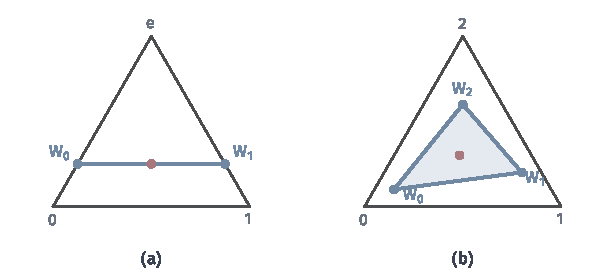
\includegraphics[width=104mm]{figures/07-probability/06-channel-coding/matplotlib/dcc-output-simplex/figure.pdf}
 \caption{输出分布的可达范围。三角形是三个输出上的概率单纯形，顶点是集中于单个输出的分布。(a) 二元擦除信道$\varepsilon=0.25$，蓝点是转移矩阵的两行，蓝线段是$q\bm{W}$的全部可能值；(b) 一个三输入三输出信道，三行为$(0.8,0.1,0.1)$、$(0.1,0.7,0.2)$、$(0.2,0.2,0.6)$，可达的输出分布是浅蓝三角形。红点是均匀输入对应的输出分布。}
 \label{fig:dcc-output-simplex}
\end{BookInlineFigure}

\paragraph{多次使用：无记忆}
传输消息时信道被使用$n$次，输入块$x^n=(x_1,\dots,x_n)$，输出块$y^n=(y_1,\dots,y_n)$。最简单的多次使用规律是：每次使用都经过同一个转移矩阵，各次之间互不影响。

\begin{definition}[离散无记忆信道]
\label{def:dcc-dmc}
以$\bm{W}$为转移矩阵的\term{离散无记忆信道}（discrete memoryless channel）在$n$次使用中，对每个输入块$x^n\in\mathcal{X}^n$，输出块的条件概率为
\begin{equation}
 W^n(y^n\mid x^n)=\prod_{i=1}^{n}W(y_i\mid x_i),\qquad y^n\in\mathcal{Y}^n .
 \label{eq:dcc-memoryless}
\end{equation}
\end{definition}

乘积形式包含两层意思：第$i$个输出只受第$i$个输入影响；给定整个输入块后，各个输出相互独立。以$p=0.1$的二元对称信道为例，发送$111$而收到$101$，需要第一、三位不翻转、第二位翻转，概率是
\[
 W^3(101\mid111)=0.9\times0.1\times0.9=0.081 .
\]

\paragraph{编码器不使用反馈}
式~\eqref{eq:dcc-memoryless}描述的是给定输入块之后输出的规律。还需要说明输入块怎样产生。本章中，发送端在传输之前就由消息确定整个输入块，第$i$次的输入不依赖已经收到的$y_1,\dots,y_{i-1}$。若发送端能看到输出（称为反馈），它可以根据前面的结果调整后面的输入，这时$X_i$与此前的噪声相关，式~\eqref{eq:dcc-memoryless}的乘积结构仍描述每一步的转移，但输入与输出的联合规律不再能直接按块写出，第~\ref{sec:dcc-capacity-formula}节的块互信息上界需要另行论证。图~\ref{fig:dcc-block-system}画出本章的传输结构。

\begin{BookInlineFigure}
 \centering
 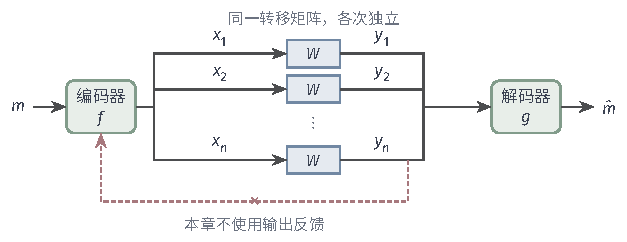
\includegraphics[width=106.2mm]{figures/07-probability/06-channel-coding/tikz/dcc-block-system/figure.pdf}
 \caption{离散无记忆信道上的块传输。编码器$f$把消息$m$一次变成整个输入块，每个符号独立地经过同一转移矩阵$W$，解码器$g$看到整个输出块后给出判决$\hat{m}$。红色虚线表示从输出到编码器的反馈，本章不使用。}
 \label{fig:dcc-block-system}
\end{BookInlineFigure}

无记忆是一个模型假设。若干扰成串出现，例如一次翻转之后紧接着的几个符号也更容易翻转，各次使用就不独立，式~\eqref{eq:dcc-memoryless}不成立。这样的信道需要随机过程的工具描述状态的演化，本章不讨论。


\section{块码}
\label{sec:dcc-block-codes}

一个比特直接送进翻转概率$p=0.1$的二元对称信道，出错的概率就是$0.1$。降低错误的朴素办法是重复：要发$0$就连发$000$，要发$1$就连发$111$，接收端看三个符号中哪个占多数。只有至少两个符号被翻转时才判错，这比单个符号翻转少见得多。

这个例子包含了信道编码的全部要素：消息不是逐个符号送出的，而是先被映成一整块输入；块中的冗余让接收端在部分符号出错时仍能判断发送的是哪条消息。本节把这些要素写成定义，规定码率与错误概率的口径。后面的容量定理和第~\ref{chap:channel-codes}章的具体纠错码都使用这里的口径。

\subsection{编码器与解码器}
\label{sec:dcc-encoder-decoder}

设要传送的消息取自有限集合$\{1,\dots,M\}$，信道使用$n$次。编码就是给每条消息指定一个长度为$n$的输入块，解码就是根据收到的输出块猜出消息。

\begin{definition}[块码]
\label{def:dcc-block-code}
离散信道上的一个$(M,n)$\term{块码}（block code）由两部分组成：
\begin{itemize}
 \item 编码器$f:\{1,\dots,M\}\to\mathcal{X}^n$，记$x^n(m)=f(m)$，称为消息$m$的码字，全部码字组成码本；
 \item 解码器$g:\mathcal{Y}^n\to\{1,\dots,M\}$，把每个输出块判为一条消息。
\end{itemize}
码的码率定义为
\begin{equation}
 R=\frac{\log_2M}{n}\quad\text{比特每次信道使用}.
 \label{eq:dcc-rate}
\end{equation}
\end{definition}

$\log_2M$是从$M$条消息中选出一条所需的比特数，除以$n$就是平均每次使用信道承载的比特数。码率最高为$\log_2\lvert\mathcal{X}\rvert$，此时$M=\lvert\mathcal{X}\rvert^n$，每个输入块都是码字，没有任何冗余。

\paragraph{三次重复码}
\term{重复码}（repetition code）中$M=2$，$n=3$。把消息记作$0$与$1$，码字是$000$与$111$，码率为$\tfrac13$。解码器采用\term{多数判决}（majority decoding）：输出块中$1$多于$0$时判为$1$，否则判为$0$。下面走一遍传输过程，区分四个对象：
\begin{enumerate}
 \item 消息：$m=1$，这是要传的内容；
 \item 码字：$x^3(1)=111$，这是送进信道的输入块；
 \item 输出块：信道翻转了第二位，接收端收到$y^3=101$；
 \item 判决：$101$中有两个$1$，$g(101)=1$，判决$\hat{m}=1$与消息一致。
\end{enumerate}
消息与判决属于消息集合，码字与输出块属于符号块；错误指的是判决与消息不同，而不是输出块与码字不同。这次传输中输出块有一位错了，判决仍然正确。

图~\ref{fig:dcc-repetition-cube}把长度为$3$的全部$8$个输出块画成立方体的顶点，相邻顶点只差一位。两个码字在相对的两个角上，多数判决把立方体分成两半：离$000$较近的四个顶点判为$0$，离$111$较近的四个判为$1$。从$111$出发翻转一位只能走到黄色顶点，所以单个翻转总能被纠正。

\begin{BookInlineFigure}
 \centering
 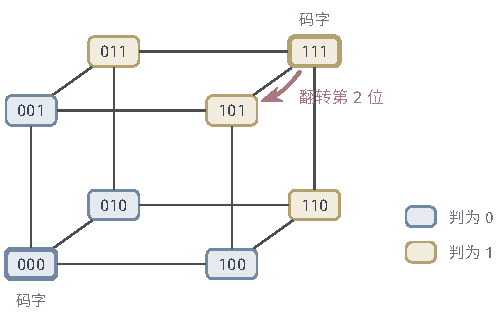
\includegraphics[width=85.4mm]{figures/07-probability/06-channel-coding/tikz/dcc-repetition-cube/figure.pdf}
 \caption{长度为$3$的输出块构成立方体的顶点，相邻顶点只差一位。粗框为码字$000$与$111$；蓝色顶点（至多一个$1$）判为$0$，黄色顶点（至少两个$1$）判为$1$。红色箭头是正文的例子：发送$111$，第二位翻转，收到$101$，判为$1$。}
 \label{fig:dcc-repetition-cube}
\end{BookInlineFigure}

在翻转概率$p=0.1$的二元对称信道上，发送$111$而判错，需要至少两位翻转。恰好两位翻转有$3$种位置，三位全翻有$1$种，所以
\[
 \mathbb{P}(\text{判错})=3p^2(1-p)+p^3=3\times0.01\times0.9+0.001=0.028 .
\]
由对称性，发送$000$时判错的概率也是$0.028$。

\paragraph{最好的解码器}
码本给定以后，解码器还可以自由选择。若每条消息以相同的概率$1/M$出现，判对的概率是
\[
 \frac1M\sum_{m=1}^{M}\ \sum_{y^n:\,g(y^n)=m}W^n\bigl(y^n\mid x^n(m)\bigr)
 =\frac1M\sum_{y^n\in\mathcal{Y}^n}W^n\bigl(y^n\mid x^n(g(y^n))\bigr) .
\]
右边对每个输出块分别求和，因此逐项取最大即可：对每个$y^n$，让$g(y^n)$取使$W^n(y^n\mid x^n(m))$最大的$m$（并列时任取其一）。这样的判决规则称为\term{最大似然解码}（maximum-likelihood decoding），它使均匀消息下的错误概率最小。在$p<\tfrac12$的二元对称信道上，$W^n(y^n\mid x^n)=p^{k}(1-p)^{n-k}$，其中$k$是$y^n$与$x^n$不同的位置数；因为$p/(1-p)<1$，似然随$k$增大而减小，最大似然就是选与输出块差异位置最少的码字。对重复码，这正是多数判决。

\subsection{错误概率与可达速率}
\label{sec:dcc-error-and-rates}

重复码的例子已经给出一个错误概率，但一般的码中，不同消息被判错的概率可以不同。为此先对每条消息定义条件错误概率，再用两种方式汇总。

\begin{definition}[错误概率]
\label{def:dcc-error-probabilities}
对$(M,n)$码，消息$m$的条件错误概率是
\begin{equation}
 \lambda_m=\mathbb{P}\bigl(g(Y^n)\neq m\mid X^n=x^n(m)\bigr)=\sum_{y^n:\,g(y^n)\neq m}W^n\bigl(y^n\mid x^n(m)\bigr) .
 \label{eq:dcc-lambda}
\end{equation}
\term{平均错误概率}（average error probability）与\term{最大错误概率}（maximal error probability）分别为
\begin{equation}
 P_{\mathrm{e}}=\frac1M\sum_{m=1}^{M}\lambda_m,\qquad \lambda_{\max}=\max_{1\leq m\leq M}\lambda_m .
 \label{eq:dcc-pe}
\end{equation}
\end{definition}

若消息$M$在$\{1,\dots,M\}$上均匀分布，$P_{\mathrm{e}}$就是判错的概率$\mathbb{P}(g(Y^n)\neq M)$。这里用同一字母$M$表示消息变量和消息个数，下文由上下文区分。$\lambda_{\max}$不依赖消息的分布，它保证每条消息都很少出错。平均不超过最大值，所以$P_{\mathrm{e}}\leq\lambda_{\max}$；第~\ref{sec:dcc-max-error}小节会说明，在渐近意义下两种口径给出相同的速率极限。

\paragraph{可达速率}
在二元对称信道这类每个输出块都可能来自任一码字的信道上，有限码的错误概率总是正的，所以“可靠”只能在码长增长的极限中定义：要求一列码的错误趋于零，同时码率不低于给定的值。

\begin{definition}[可达速率与容量]
\label{def:dcc-achievable}
称$R\geq0$为\term{可达速率}（achievable rate），若存在一列$(M_n,n)$码，满足
\begin{equation}
 M_n\geq2^{nR},\qquad \lim_{n\to\infty}P_{\mathrm{e}}^{(n)}=0 ,
 \label{eq:dcc-achievable}
\end{equation}
其中$P_{\mathrm{e}}^{(n)}$是第$n$个码的平均错误概率。可达速率的上确界称为信道的\term{信道容量}（channel capacity），记作$C_{\mathrm{op}}$。
\end{definition}

$R=0$总是可达的：取$M_n=1$，只有一条消息，解码器永远判对。可达速率的集合是区间：若$R$可达，比它小的速率用同一列码即可满足$M_n\geq2^{nR'}$。下标“op”表示这个容量是按传输任务定义的；下一节给出一个由信道直接计算的量，第~\ref{sec:dcc-coding-theorem}节证明二者相等。

\paragraph{重复码不够}
长度为奇数$n$的重复码在$p=0.1$的二元对称信道上，判错的概率是$\mathrm{Bin}(n,0.1)$至少取到$(n+1)/2$的概率。由第~\ref{chap:laws-of-large-numbers}章的弱大数律，翻转比例趋于$0.1<\tfrac12$，这个概率趋于零。可是码率$1/n$也趋于零，所以重复码只说明速率$0$可达。图~\ref{fig:dcc-repetition-error}画出前几个重复码：错误按指数下降，但它们在码率—错误平面上全部挤向纵轴，远离$C\approx0.531$。

\begin{BookInlineFigure}
 \centering
 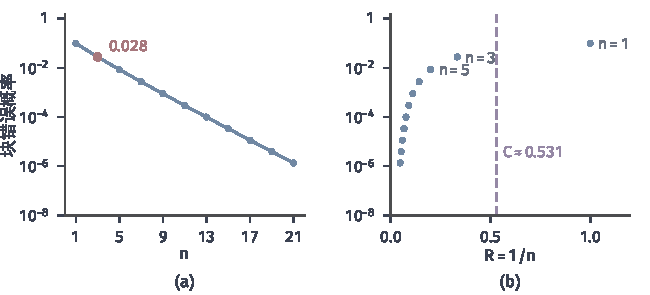
\includegraphics[width=110mm]{figures/07-probability/06-channel-coding/matplotlib/dcc-repetition-error/figure.pdf}
 \caption{翻转概率$0.1$的二元对称信道上，奇数长度$n$的重复码配合多数判决。(a) 块错误概率随$n$的精确值，对数坐标，红点为$n=3$时的$0.028$；(b) 同一组码在码率—错误平面上的位置，码率为$1/n$，紫色虚线为第~\ref{sec:dcc-bsc}小节算出的容量$0.531$。}
 \label{fig:dcc-repetition-error}
\end{BookInlineFigure}

图中$n=1$的“码”码率为$1$，超过了容量，错误概率却只有$0.1$。这并不矛盾：容量限制的是错误能否趋于零，对单个有限码的错误概率没有直接要求。反过来也一样，速率低于容量只保证存在错误趋于零的码列，并不保证某个有限长度的码错误为零。可达速率是关于码长增长时的极限陈述，有限长度需要多少冗余由第~\ref{chap:channel-codes}章讨论。


\section{容量公式}
\label{sec:dcc-capacity-formula}

可达速率的定义涉及所有码长、所有码本与所有解码器，直接求其上确界无从下手。本节从信道本身构造一个可以计算的量，并证明它控制任意长度输入块能获得的信息。下一节再证明它就是$C_{\mathrm{op}}$。

\paragraph{计数的图景}
先用一个粗略的计数说明为什么应当看互信息。设输入块的各符号按分布$q$独立选取，输出块也就按$p_q$独立分布。由第~\ref{chap:lossless-coding}章的典型集合，输出块几乎总落在约$2^{nH(Y)}$个“典型”输出块之中；给定一个码字，信道噪声使输出块落在约$2^{nH(Y\mid X)}$个块组成的小范围内。若要从输出块唯一认出码字，各码字的小范围应当基本不重叠，于是码字数至多约为
\[
 \frac{2^{nH(Y)}}{2^{nH(Y\mid X)}}=2^{n\,(H(Y)-H(Y\mid X))}=2^{nI(X;Y)} .
\]
每次使用约承载$I(X;Y)$比特。图~\ref{fig:dcc-typical-fans}画出这幅图景。它是启发，不是证明：“约”字隐去了误差，小范围之间也不必完全不交。第~\ref{sec:dcc-coding-theorem}节把这个计数做成严格的论证。

\begin{BookInlineFigure}
 \centering
 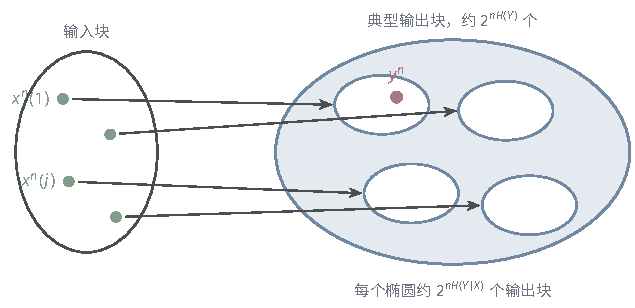
\includegraphics[width=107.5mm]{figures/07-probability/06-channel-coding/tikz/dcc-typical-fans/figure.pdf}
 \caption{容量公式背后的计数。左侧绿点是按输入分布选出的码字；右侧蓝色区域是约$2^{nH(Y)}$个典型输出块，每个码字经过信道后的可能输出集中在约$2^{nH(Y\mid X)}$个块组成的小椭圆中。红点是收到的输出块，它落在所发码字的椭圆内。互不重叠的椭圆至多约有$2^{nI(X;Y)}$个。}
 \label{fig:dcc-typical-fans}
\end{BookInlineFigure}

\paragraph{互信息作为输入分布的函数}
固定信道$\bm{W}$，输入分布为$q$时，第~\ref{chap:information-measures}章的互信息（以比特计）是
\[
 I(X;Y)=\sum_{x,y}q(x)W(y\mid x)\log_2\frac{W(y\mid x)}{p_q(y)} ,
\]
求和只取$q(x)W(y\mid x)>0$的项，此时$p_q(y)\geq q(x)W(y\mid x)>0$，每项都有定义。字母表有限，所以各个熵都有限，并且$I(X;Y)=H(Y)-H(Y\mid X)$。按输入分组，内层和正是第$x$行相对于输出分布的KL散度，于是
\begin{equation}
 I(q)=\sum_{x\in\mathcal{X}}q(x)\,D_{\mathrm{KL}}\bigl(W_x\Vert p_q\bigr) .
 \label{eq:dcc-mi-divergence}
\end{equation}
这里把互信息写成$I(q)$，强调信道固定后它只是$q$的函数。式~\eqref{eq:dcc-mi-divergence}的读法是：每个输入$x$的输出分布偏离总体输出分布越远，用$x$传递的信息越多；互信息是这些偏离按使用频率的平均。

\begin{definition}[信息容量]
\label{def:dcc-information-capacity}
离散信道$\bm{W}$的信息容量是
\begin{equation}
 C=\max_{q\in\Delta_{\mathcal{X}}}I(q) .
 \label{eq:dcc-capacity}
\end{equation}
达到最大值的$q$称为最优输入分布。
\end{definition}

定义中写的是最大值而不是上确界，需要说明它能取到；同时，最优输入分布怎样刻画，也决定了后面的计算方法。

\begin{theorem}[容量的存在与凹性]
\label{thm:dcc-capacity-exists}
$I(q)$是单纯形$\Delta_{\mathcal{X}}$上的连续凹函数。因此式~\eqref{eq:dcc-capacity}的最大值存在，并且
\begin{equation}
 0\leq C\leq\min\bigl\{\log_2\lvert\mathcal{X}\rvert,\ \log_2\lvert\mathcal{Y}\rvert\bigr\} ;
 \label{eq:dcc-capacity-range}
\end{equation}
最优输入分布组成凸集，所有最优输入分布给出同一个输出分布。
\end{theorem}

\begin{proof}
把互信息写成熵差：
\[
 I(q)=H(p_q)-\sum_{x}q(x)H(W_x) ,
\]
其中$H(p_q)=\sum_y\varphi(p_q(y))$，$\varphi(t)=-t\log_2t$（$\varphi(0)=0$）。$\varphi$在$[0,1]$上连续，$p_q$是$q$的线性函数，所以$H(p_q)$关于$q$连续；第二项是$q$的线性函数。于是$I$连续。

凹性。第~\ref{chap:information-measures}章证明了熵是概率分布的凹函数，而且因为$\varphi$严格凹，这种凹性是严格的：$p\neq p'$时，对$0<\theta<1$有$H(\theta p+(1-\theta)p')>\theta H(p)+(1-\theta)H(p')$。$q\mapsto p_q$是线性的，凹函数与线性映射的复合仍是凹函数；减去一个线性函数不改变凹性。所以$I$凹。

$\Delta_{\mathcal{X}}$是有界闭集，连续函数在其上取到最大值。凹函数在凸集上的最大值点组成凸集：若$q_1,q_2$都达到$C$，则对$\theta\in[0,1]$，
\[
 I\bigl(\theta q_1+(1-\theta)q_2\bigr)\geq\theta C+(1-\theta)C=C .
\]
若两者的输出分布不同，由$H$的严格凹性，中点处的不等式是严格的，$I$会超过$C$，这不可能。所以最优输出分布唯一。

上界：$I(X;Y)\leq H(X)\leq\log_2\lvert\mathcal{X}\rvert$，同理$I(X;Y)\leq H(Y)\leq\log_2\lvert\mathcal{Y}\rvert$；下界由互信息非负得到。
\end{proof}

凹性带来的好处是局部最优就是全局最优，最优输入可以用一阶条件刻画。凹性本身不保证最优输入唯一：例如两个输入的转移行完全相同时，它们之间的分配可以任意调换。

\paragraph{例：Z信道}
Z信道中记$q=\mathbb{P}(X=1)$。输出为$1$当且仅当输入为$1$且没有出错，所以$p_q(1)=q/2$。给定$X=0$时输出确定，熵为$0$；给定$X=1$时输出是公平硬币，熵为$1$比特。于是
\[
 I(q)=h_2\Bigl(\frac q2\Bigr)-q ,
\]
其中$h_2(t)=-t\log_2t-(1-t)\log_2(1-t)$是二元熵函数。对$q$求导，$h_2'(t)=\log_2\frac{1-t}{t}$，得到
\[
 I'(q)=\frac12\log_2\frac{2-q}{q}-1 .
\]
令它为零，得$(2-q)/q=4$，即$q=\tfrac25$。代回，$h_2(\tfrac15)=\log_25-\tfrac85$，所以
\[
 C=\log_25-\frac85-\frac25=\log_2\frac54\approx0.3219 .
\]
最优输入并不均匀：输入$1$会以一半的概率被误读成$0$，少用一些更划算。均匀输入时$I(\tfrac12)=h_2(\tfrac14)-\tfrac12\approx0.3113$，比容量少约$0.011$比特。图~\ref{fig:dcc-mi-curves}把它与两个对称信道的$I(q)$画在一起。

\begin{BookInlineFigure}
 \centering
 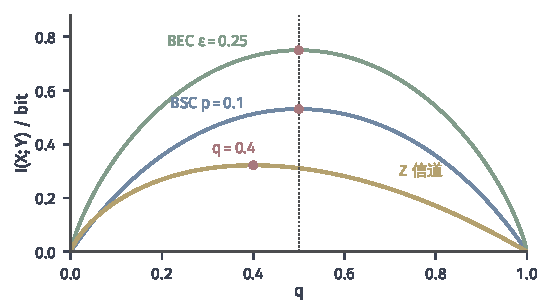
\includegraphics[width=92mm]{figures/07-probability/06-channel-coding/matplotlib/dcc-mi-curves/figure.pdf}
 \caption{三个二元输入信道的互信息随输入概率$q=\mathbb{P}(X=1)$的变化：蓝线为翻转概率$0.1$的二元对称信道，绿线为擦除概率$0.25$的二元擦除信道，黄线为Z信道。三条曲线都是凹的，红点为最大值即容量；两个对称信道在$q=\tfrac12$处取最大值，Z信道在$q=0.4$处取最大值$\log_2(5/4)$。}
 \label{fig:dcc-mi-curves}
\end{BookInlineFigure}

\paragraph{最优性条件}
对二元输入，一元求导就能找到最大值；输入多于两个时，需要一个对单纯形上的点都适用的判别法。式~\eqref{eq:dcc-mi-divergence}提示：最优时，凡是被使用的输入，其“信息贡献”$D_{\mathrm{KL}}(W_x\Vert p_q)$应当相等，否则把概率从贡献小的输入挪到贡献大的输入就能增加互信息。下面的定理把这一想法写准确，并顺带给出一个任何时候都能算的上界。

\begin{theorem}[容量的上界与最优性条件]
\label{thm:dcc-kkt}
\begin{enumerate}
 \item 对$\mathcal{Y}$上的任意概率分布$r$，
 \begin{equation}
  C\leq\max_{x\in\mathcal{X}}D_{\mathrm{KL}}\bigl(W_x\Vert r\bigr) .
  \label{eq:dcc-upper-bound}
 \end{equation}
 \item $q^{*}\in\Delta_{\mathcal{X}}$是最优输入分布，当且仅当存在常数$c$，使得记$p^{*}=p_{q^{*}}$时
 \begin{equation}
  D_{\mathrm{KL}}\bigl(W_x\Vert p^{*}\bigr)=c\ \ \text{若}\ q^{*}(x)>0,\qquad D_{\mathrm{KL}}\bigl(W_x\Vert p^{*}\bigr)\leq c\ \ \text{若}\ q^{*}(x)=0 .
  \label{eq:dcc-kkt}
 \end{equation}
 此时$c=C$。
\end{enumerate}
\end{theorem}

\begin{proof}
先证一个恒等式。对任意$q$与任意$r$，把$\log_2(W/r)$拆成$\log_2(W/p_q)+\log_2(p_q/r)$，得到
\[
 \sum_{x}q(x)D_{\mathrm{KL}}(W_x\Vert r)=\sum_xq(x)D_{\mathrm{KL}}(W_x\Vert p_q)+\sum_{y}p_q(y)\log_2\frac{p_q(y)}{r(y)} ,
\]
其中用到$\sum_xq(x)W(y\mid x)=p_q(y)$。由式~\eqref{eq:dcc-mi-divergence}，右边是$I(q)+D_{\mathrm{KL}}(p_q\Vert r)$。若某项为无穷，等式两边同为无穷。于是
\[
 I(q)=\sum_xq(x)D_{\mathrm{KL}}(W_x\Vert r)-D_{\mathrm{KL}}(p_q\Vert r)\leq\max_xD_{\mathrm{KL}}(W_x\Vert r) .
\]
对$q$取最大值就得到式~\eqref{eq:dcc-upper-bound}。

充分性。设式~\eqref{eq:dcc-kkt}成立。由式~\eqref{eq:dcc-mi-divergence}，$I(q^{*})$是$D_{\mathrm{KL}}(W_x\Vert p^{*})$在$q^{*}$支撑上的平均，等于$c$。取$r=p^{*}$，式~\eqref{eq:dcc-upper-bound}给出$C\leq c$。所以$I(q^{*})=c\geq C$，$q^{*}$最优且$c=C$。

必要性。设$q^{*}$最优，任取$x'\in\mathcal{X}$，令$q_t=(1-t)q^{*}+t\,\delta_{x'}$，$t\in[0,1]$，其中$\delta_{x'}$是集中在$x'$的分布。先设$W_{x'}$的支撑包含在$p^{*}$的支撑中。对$I(q_t)=H(p_{q_t})-\sum_xq_t(x)H(W_x)$在$t=0$处求右导数，$p_{q_t}=p^{*}+t(W_{x'}-p^{*})$，熵项的导数是
\[
 \begin{aligned}
 &-\sum_{y}\bigl(W(y\mid x')-p^{*}(y)\bigr)\Bigl(\log_2p^{*}(y)+\frac{1}{\ln2}\Bigr)\\
 &\qquad=-\sum_yW(y\mid x')\log_2p^{*}(y)-H(p^{*}) ,
 \end{aligned}
\]
这里只对$p^{*}(y)>0$的$y$求和，$\sum_y(W(y\mid x')-p^{*}(y))=0$消去了常数项。线性项的导数是$-H(W_{x'})+\sum_xq^{*}(x)H(W_x)$。两部分相加，得到
\[
 \frac{\mathrm{d}}{\mathrm{d}t}I(q_t)\Big|_{t=0^{+}}=D_{\mathrm{KL}}(W_{x'}\Vert p^{*})-I(q^{*}) .
\]
$q^{*}$是最大值点，右导数不能为正，所以$D_{\mathrm{KL}}(W_{x'}\Vert p^{*})\leq I(q^{*})=C$。若$W_{x'}$在某个$p^{*}(y)=0$的$y$上有正质量，则$p_{q_t}(y)=tW(y\mid x')$，熵中这一项$-tW\log_2(tW)$的右导数为$+\infty$，其余项导数有限，$I(q_t)$在$t=0$附近严格增加，与最优性矛盾；所以这种情形不会出现。于是对一切$x'$有$D_{\mathrm{KL}}(W_{x'}\Vert p^{*})\leq C$；而这些散度按$q^{*}$的平均等于$C$，所以在支撑上必须取等号。
\end{proof}

式~\eqref{eq:dcc-kkt}是卷五中约束优化一阶条件在单纯形上的具体形式：等式约束$\sum_xq(x)=1$的乘子是$c$，非负约束在$q^{*}(x)=0$处起作用，允许不等号，可参考\BookChapterRef{chap:constrained-optimality}{卷五第17章“约束问题的最优性”}。上界~\eqref{eq:dcc-upper-bound}对任意$r$成立，不需要知道最优输入；第~\ref{sec:dcc-numerical}节用它作为数值计算的停止依据。

用Z信道检验条件~\eqref{eq:dcc-kkt}。$q^{*}=(\tfrac35,\tfrac25)$时$p^{*}=(\tfrac45,\tfrac15)$，两行的散度为
\[
 \begin{aligned}
 D_{\mathrm{KL}}(W_0\Vert p^{*})&=\log_2\frac{1}{4/5}=\log_2\frac54 ,\\
 D_{\mathrm{KL}}(W_1\Vert p^{*})&=\frac12\log_2\frac{1/2}{4/5}+\frac12\log_2\frac{1/2}{1/5}=\frac12\log_2\frac{25}{16}=\log_2\frac54 .
 \end{aligned}
\]
两者相等，都等于容量。

\paragraph{块的互信息不超过单次容量的$n$倍}
容量是单次使用的量，传输却用整块输入。块输入的各符号可以按任意方式相关，例如重复码让三个符号完全相同。这种相关能否让$n$次使用获得多于$nC$的信息？下面的引理说不能，并且独立使用最优输入恰好达到$nC$。

\begin{lemma}[块互信息的单次上界]
\label{lem:dcc-block-bound}
设$X^n=(X_1,\dots,X_n)$在$\mathcal{X}^n$上有任意分布，给定$X^n=x^n$时$Y^n$的条件分布由式~\eqref{eq:dcc-memoryless}给出。则
\begin{equation}
 I(X^n;Y^n)\leq\sum_{i=1}^{n}I(X_i;Y_i)\leq nC .
 \label{eq:dcc-block-bound}
\end{equation}
若$X_1,\dots,X_n$独立且都服从最优输入分布，则两处都取等号。
\end{lemma}

\begin{proof}
先算条件熵。对式~\eqref{eq:dcc-memoryless}中$j\neq i$的坐标求和，每个因子$\sum_{y_j}W(y_j\mid x_j)=1$，得到$\mathbb{P}(Y_i=y\mid X^n=x^n)=W(y\mid x_i)$：$(X_i,Y_i)$的联合分布是$X_i$的边缘分布乘以$\bm{W}$。取对数，乘积变成和：
\[
 \begin{aligned}
 H(Y^n\mid X^n)&=\mathbb{E}\bigl[-\log_2W^n(Y^n\mid X^n)\bigr]\\
 &=\sum_{i=1}^{n}\mathbb{E}\bigl[-\log_2W(Y_i\mid X_i)\bigr]=\sum_{i=1}^{n}H(Y_i\mid X_i) .
 \end{aligned}
\]
再看输出熵。由熵的链式法则与“条件化不增加熵”，
\[
 H(Y^n)=\sum_{i=1}^{n}H(Y_i\mid Y_1,\dots,Y_{i-1})\leq\sum_{i=1}^{n}H(Y_i) .
\]
两式相减，
\[
 \begin{aligned}
 I(X^n;Y^n)&=H(Y^n)-H(Y^n\mid X^n)\\
 &\leq\sum_{i=1}^{n}\bigl(H(Y_i)-H(Y_i\mid X_i)\bigr)=\sum_{i=1}^{n}I(X_i;Y_i) .
 \end{aligned}
\]
每个$I(X_i;Y_i)$是$X_i$的边缘分布对应的互信息，不超过$C$。

若$X_i$独立同服从最优分布$q^{*}$，则联合概率$\prod_iq^{*}(x_i)W(y_i\mid x_i)$分解为$n$个相同因子的乘积，$(X_i,Y_i)$相互独立，$Y_1,\dots,Y_n$也相互独立，于是$H(Y^n)=\sum_iH(Y_i)$，且每个$I(X_i;Y_i)=C$。
\end{proof}

图~\ref{fig:dcc-memoryless-graph}画出证明所用的依赖结构。条件熵能够精确相加，是因为每个输出只通过自己的输入受影响；输出熵只能放大成和，是因为各输出可能经由输入彼此相关。输入之间的相关只会让$H(Y^n)$变小，不会让信息变多：重复码的三个输出高度相关，所以三次使用得到的信息远少于$3C$。

\begin{BookInlineFigure}
 \centering
 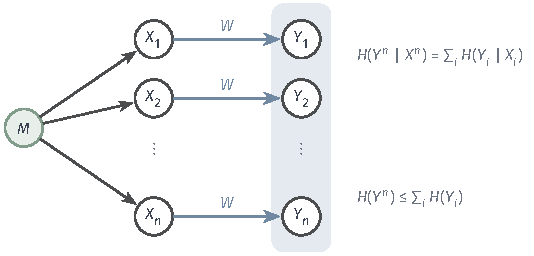
\includegraphics[width=90.5mm]{figures/07-probability/06-channel-coding/tikz/dcc-memoryless-graph/figure.pdf}
 \caption{无反馈块传输的依赖结构。消息$M$决定整个输入块，各输入可以经由$M$相关；每个输出$Y_i$只由$X_i$经过同一个$W$产生。条件熵因此精确相加，而浅蓝色框内的输出可能彼此相关，输出熵只满足次可加不等式。}
 \label{fig:dcc-memoryless-graph}
\end{BookInlineFigure}

引理只说块输入能获得的信息至多为$nC$，还没有说明这些信息能被一个码本和一个解码器实际兑现成低错误的消息传输，也没有说明信息上界为什么限制码率。这两个方向分别是下一节的可达性与逆定理。


\section{信道编码定理}
\label{sec:dcc-coding-theorem}

现在有两个“容量”：按传输任务定义的$C_{\mathrm{op}}$，即错误能趋于零的码率的上确界；以及式~\eqref{eq:dcc-capacity}中由转移矩阵算出的$C$。引理~\ref{lem:dcc-block-bound}说明$n$次使用至多获得$nC$比特信息，计数图景又提示$2^{nC}$条消息大致能被区分。下面的定理说两者相等。

\begin{theorem}[信道编码定理]
\label{thm:dcc-coding-theorem}
对有限字母表上的离散无记忆信道（编码器不使用反馈），
\begin{equation}
 C_{\mathrm{op}}=C=\max_{q\in\Delta_{\mathcal{X}}}I(q) .
 \label{eq:dcc-coding-theorem}
\end{equation}
具体地说：每个$R<C$都是可达速率，并且可以要求最大错误概率趋于零；每个$R>C$都不是可达速率。
\end{theorem}

定理由两个方向组成。可达性（第~\ref{sec:dcc-achievability}小节）是存在性陈述：码率低于容量时，存在错误趋于零的码列。逆定理（第~\ref{sec:dcc-converse}小节）是必要性陈述：码率高于容量时，任何码列的错误都不能趋于零。定理对$R=C$本身不作断言，也不说某个有限长度的码已经可靠；它描述的是码长增长时能够逼近的速率边界。这一陈述最早由Shannon给出，完整的历史与推广可查阅~\scite{math-cover2006information}。

\subsection{随机编码的可达性}
\label{sec:dcc-achievability}

要证明可达，需要对每个$R<C$造出一列码。直接构造很难，证明采用一个间接办法：随机抽取码本，证明随机码本的平均错误概率趋于零，于是必有某个具体码本不比平均差。解码器则用“联合典型性”判断一个码字与输出块是否匹配。

\paragraph{联合典型集}
设$(X,Y)$的联合分布为$q(x)W(y\mid x)$，输出分布为$p=p_q$。把$n$个独立同分布的对$(X_i,Y_i)$排成块，块的概率是单个概率的乘积，记作$q^n(x^n)=\prod_iq(x_i)$，$p^n(y^n)=\prod_ip(y_i)$，以及$P^n(x^n,y^n)=\prod_iq(x_i)W(y_i\mid x_i)$。由第~\ref{chap:laws-of-large-numbers}章的大数律，$-\frac1n\log_2q^n(X^n)$是$n$个独立同分布的$-\log_2q(X_i)$的平均，会集中到它的均值$H(X)$。联合典型集把这种集中同时要求在三个层面上。

\begin{definition}[联合典型集]
\label{def:dcc-joint-typical}
给定$\epsilon>0$，\term{联合典型集}（jointly typical set）$A_{\epsilon}^{(n)}$由满足下面三个条件的$(x^n,y^n)\in\mathcal{X}^n\times\mathcal{Y}^n$组成：
\begin{equation}
 \begin{aligned}
 \Bigl\lvert-\tfrac1n\log_2q^n(x^n)-H(X)\Bigr\rvert&<\epsilon ,\\
 \Bigl\lvert-\tfrac1n\log_2p^n(y^n)-H(Y)\Bigr\rvert&<\epsilon ,\\
 \Bigl\lvert-\tfrac1n\log_2P^n(x^n,y^n)-H(X,Y)\Bigr\rvert&<\epsilon .
 \end{aligned}
 \label{eq:dcc-joint-typical}
\end{equation}
概率为零的块，其负对数视为$+\infty$，不属于$A_{\epsilon}^{(n)}$。
\end{definition}

直观上，联合典型的一对块“看起来像”由这条信道产生的：输入块的组成像$q$，输出块的组成像$p$，两者之间的对应关系像$\bm{W}$。下面的引理给出三条性质，分别对应计数图景中的三个“约”字。

\begin{lemma}[联合典型性]
\label{lem:dcc-joint-aep}
\begin{enumerate}
 \item 若$(X_i,Y_i)$独立同服从$q(x)W(y\mid x)$，则当$n\to\infty$时
 \begin{equation}
  \mathbb{P}\bigl((X^n,Y^n)\in A_{\epsilon}^{(n)}\bigr)\to1 .
  \label{eq:dcc-typical-prob}
 \end{equation}
 \item 典型集的元素个数满足
 \begin{equation}
  \bigl\lvert A_{\epsilon}^{(n)}\bigr\rvert\leq2^{n(H(X,Y)+\epsilon)} .
  \label{eq:dcc-typical-size}
 \end{equation}
 \item 若$\tilde{X}^n\sim q^n$与$\tilde{Y}^n\sim p^n$相互独立，则
 \begin{equation}
  \mathbb{P}\bigl((\tilde{X}^n,\tilde{Y}^n)\in A_{\epsilon}^{(n)}\bigr)\leq2^{-n(I(X;Y)-3\epsilon)} .
  \label{eq:dcc-independent-typical}
 \end{equation}
\end{enumerate}
\end{lemma}

\begin{proof}
(1) 以概率$1$，每个$X_i$取$q(x)>0$的值，每对取正概率的值，所以$-\log_2q(X_i)$、$-\log_2p(Y_i)$、$-\log_2[q(X_i)W(Y_i\mid X_i)]$都是有界的随机变量，均值分别为$H(X)$、$H(Y)$、$H(X,Y)$。块的负对数概率除以$n$恰好是它们的样本平均。由弱大数律，对每个条件，违反它的概率趋于零；三个概率之和也趋于零。

(2) 集合中每一对都满足$P^n(x^n,y^n)\geq2^{-n(H(X,Y)+\epsilon)}$，所以
\[
 1\geq\sum_{(x^n,y^n)\in A_{\epsilon}^{(n)}}P^n(x^n,y^n)\geq\bigl\lvert A_{\epsilon}^{(n)}\bigr\rvert\,2^{-n(H(X,Y)+\epsilon)} .
\]

(3) 独立的一对取值$(x^n,y^n)$的概率是$q^n(x^n)p^n(y^n)$。在$A_{\epsilon}^{(n)}$上，由前两个条件，它不超过$2^{-n(H(X)-\epsilon)}2^{-n(H(Y)-\epsilon)}$。乘以(2)中的个数，
\[
 \mathbb{P}\bigl((\tilde{X}^n,\tilde{Y}^n)\in A_{\epsilon}^{(n)}\bigr)\leq2^{n(H(X,Y)+\epsilon)}\,2^{-n(H(X)+H(Y)-2\epsilon)}=2^{-n(I(X;Y)-3\epsilon)} ,
\]
最后用到$I(X;Y)=H(X)+H(Y)-H(X,Y)$。
\end{proof}

第(1)条说正确的一对几乎总是典型的，第(3)条说无关的一对很少看起来像典型的。两条之间的差距就是解码的依据。图~\ref{fig:dcc-info-density}在翻转概率$0.1$、均匀输入的二元对称信道上画出这一差距。此时$-\frac1n\log_2q^n(x^n)=1=H(X)$对每个块都成立，输出块也一样，三个条件只剩第三个；它等价于看信息密度
\[
 \frac1n\log_2\frac{W^n(y^n\mid x^n)}{p^n(y^n)}=1+\frac kn\log_2p+\Bigl(1-\frac kn\Bigr)\log_2(1-p)
\]
是否接近$I(X;Y)=0.531$，其中$k$是$x^n$与$y^n$不同的位置数。正确的一对中$k\sim\mathrm{Bin}(n,0.1)$；独立的一对中$k\sim\mathrm{Bin}(n,\tfrac12)$，信息密度集中在$-0.737$附近。$n$增大时两团质量都收缩，彼此分离得越来越清楚。

\begin{BookInlineFigure}
 \centering
 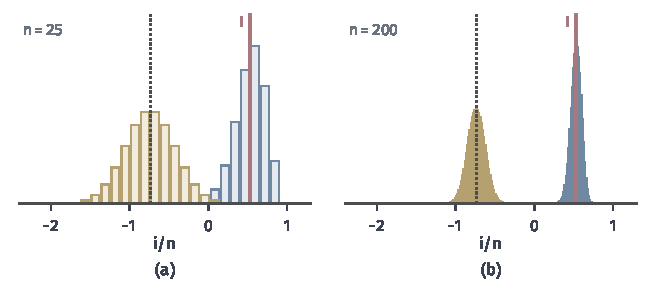
\includegraphics[width=110mm]{figures/07-probability/06-channel-coding/matplotlib/dcc-info-density/figure.pdf}
 \caption{翻转概率$0.1$的二元对称信道、均匀输入时，归一化信息密度$i/n=\frac1n\log_2[W^n(y^n\mid x^n)/p^n(y^n)]$的精确分布。蓝色为码字与其输出块的正确配对，黄色为与输出块独立的码字；红线为$I=0.531$，点线为独立配对的均值$-0.737$。(a) $n=25$；(b) $n=200$。}
 \label{fig:dcc-info-density}
\end{BookInlineFigure}

\paragraph{可达性的证明}

\begin{theorem}[可达性]
\label{thm:dcc-achievability}
对离散无记忆信道，每个$0\leq R<C$都是可达速率。
\end{theorem}

\begin{proof}
$R=0$已知可达，下设$0<R<C$。取最优输入分布$q^{*}$，于是$I(X;Y)=C$；再取$\epsilon>0$使$R<C-3\epsilon$。令$M=\lceil2^{nR}\rceil$，则$M-1<2^{nR}$。

随机码本。独立地抽取$M$个码字$\mathsf{X}^n(1),\dots,\mathsf{X}^n(M)$，每个码字的$n$个符号独立同服从$q^{*}$，即每个码字服从$(q^{*})^n$。码本抽定以后告诉收发双方，传输消息$m$时发送$\mathsf{X}^n(m)$。

解码规则。收到$y^n$后，若恰有一个$\hat{m}$使$(\mathsf{X}^n(\hat{m}),y^n)\in A_{\epsilon}^{(n)}$，就判为$\hat{m}$；否则判为$1$。

错误分析。固定消息$m$，设发送的是$\mathsf{X}^n(m)$，输出为$Y^n$。定义事件
\[
 E_j=\bigl\{(\mathsf{X}^n(j),Y^n)\in A_{\epsilon}^{(n)}\bigr\},\qquad j=1,\dots,M .
\]
若$E_m$发生而其余$E_j$都不发生，解码器判为$m$。所以判错的事件包含于$E_m^{\mathrm{c}}\cup\bigcup_{j\neq m}E_j$，由并集上界，对码本与信道噪声一起取概率，
\[
 \mathbb{E}[\lambda_m]\leq\mathbb{P}(E_m^{\mathrm{c}})+\sum_{j\neq m}\mathbb{P}(E_j) ,
\]
这里$\lambda_m$随码本而变，$\mathbb{E}$是对码本求平均。

第一项：$(\mathsf{X}^n(m),Y^n)$的各对$(X_i,Y_i)$独立同服从$q^{*}(x)W(y\mid x)$，由引理~\ref{lem:dcc-joint-aep}(1)，$\mathbb{P}(E_m^{\mathrm{c}})\to0$。

第二项：$j\neq m$时，$\mathsf{X}^n(j)$与$(\mathsf{X}^n(m),Y^n)$独立，而$Y^n$的边缘分布是$(p^{*})^n$。由式~\eqref{eq:dcc-independent-typical}，$\mathbb{P}(E_j)\leq2^{-n(C-3\epsilon)}$。合起来，
\[
 \mathbb{E}[\lambda_m]\leq\mathbb{P}(E_m^{\mathrm{c}})+(M-1)\,2^{-n(C-3\epsilon)}\leq\mathbb{P}(E_m^{\mathrm{c}})+2^{-n(C-3\epsilon-R)} .
\]
右边与$m$无关，记为$\delta_n$；因为$C-3\epsilon-R>0$，$\delta_n\to0$。

选出确定码本。对$m$取平均，随机码本的平均错误概率满足$\mathbb{E}[P_{\mathrm{e}}]\leq\delta_n$。一个随机变量不可能处处大于它的均值，所以存在某个具体码本，其平均错误概率$P_{\mathrm{e}}^{(n)}\leq\delta_n$。对每个$n$取这样一个码本，得到$M_n=\lceil2^{nR}\rceil\geq2^{nR}$且$P_{\mathrm{e}}^{(n)}\to0$的码列。
\end{proof}

为什么码率低于互信息就够了？错误有两个来源。正确码字不典型，这由大数律控制，与码率无关。某个竞争码字碰巧看起来与输出匹配，每个竞争者的机会约为$2^{-nC}$，竞争者约有$2^{nR}$个，总机会约为$2^{-n(C-R)}$；只要$R<C$，它就按指数趋于零。这正是计数图景的严格版本：小椭圆的个数$2^{nR}$少于能容纳的数目$2^{nC}$。

\paragraph{一个精确的数值}
在翻转概率$0.1$、均匀输入的二元对称信道上，证明中的两项都可以按$k$的二项分布精确求和，不必用指数上界。图~\ref{fig:dcc-random-coding-bound}画出$\mathbb{P}(E_m^{\mathrm{c}})+(M-1)\mathbb{P}(E_j)$随块长的变化（在$1$处截断），容差取$\epsilon=(C-R)/2$。$R=0.25$时，$n=1000$的值约为$4.7\times10^{-6}$，$n=2000$时约为$2.2\times10^{-10}$；$R=0.40$更靠近容量，$n=1000$时仍有$0.031$，$n=2000$时降到$0.0020$。越靠近容量，需要的块长越长。$R=0.60$高于容量，这个上界始终为$1$；下一小节证明这不只是上界的缺陷。

\begin{BookInlineFigure}
 \centering
 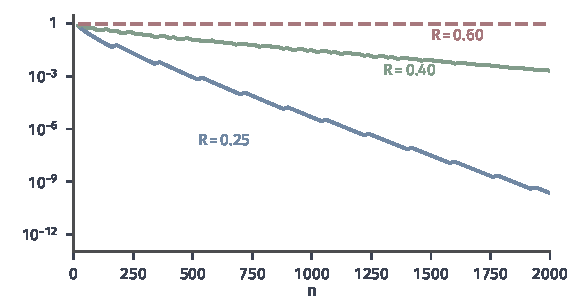
\includegraphics[width=96mm]{figures/07-probability/06-channel-coding/matplotlib/dcc-random-coding-bound/figure.pdf}
 \caption{翻转概率$0.1$的二元对称信道上随机编码的错误上界$\mathbb{P}(E_m^{\mathrm{c}})+(M-1)\mathbb{P}(E_j)$，$M=\lceil2^{nR}\rceil$，均匀输入，两项都按二项分布精确计算，值在$1$处截断，纵轴为对数坐标。蓝线$R=0.25$与绿线$R=0.40$低于容量$0.531$，容差$\epsilon=(C-R)/2$；红色虚线$R=0.60$高于容量，取$\epsilon=0.05$。曲线的小幅锯齿来自$k$的整数取值。}
 \label{fig:dcc-random-coding-bound}
\end{BookInlineFigure}

\paragraph{存在不等于可用}
证明只说明好码本存在，没有给出低成本的编码与解码。随机码本没有结构，必须整体存储$M n$个符号；典型性解码要把输出块与全部$M$个码字逐一比较。$R=0.25$、$n=1000$时，$M=2^{250}$，无论存储还是比较都无法实现。用代数结构降低编码与解码的代价，是第~\ref{chap:channel-codes}章的任务。

\subsection{逆定理}
\label{sec:dcc-converse}

可达性给出了容量以下的速率。反方向要说明：码率高于$C$时，无论码本与解码器如何设计，错误都不能趋于零。思路是把“判对”翻译成“消息与输出之间有很多信息”，再用引理~\ref{lem:dcc-block-bound}说明信息不会超过$nC$。

翻译所用的工具是第~\ref{chap:information-measures}章的Fano不等式。设消息变量取值于$M\geq2$个标签，$\hat{M}$是对它的判决，$P_{\mathrm{e}}=\mathbb{P}(\hat{M}\neq M)$。以比特计，Fano不等式为
\[
 H(M\mid\hat{M})\leq h_2(P_{\mathrm{e}})+P_{\mathrm{e}}\log_2(M-1)\leq1+P_{\mathrm{e}}\log_2M ,
\]
第二步用了$h_2\leq1$。它说判错的机会小，判决后剩余的不确定性就少。

\begin{theorem}[逆定理]
\label{thm:dcc-converse}
设$(M,n)$码用于离散无记忆信道，编码器不使用反馈，$M\geq2$，消息均匀分布。则平均错误概率满足
\begin{equation}
 P_{\mathrm{e}}\geq1-\frac{nC+1}{\log_2M} .
 \label{eq:dcc-fano-bound}
\end{equation}
特别地，若$M\geq2^{nR}$，则$P_{\mathrm{e}}\geq1-C/R-1/(nR)$；当$R>C$时，任何这样的码列都满足
\begin{equation}
 \liminf_{n\to\infty}P_{\mathrm{e}}^{(n)}\geq1-\frac CR>0 ,
 \label{eq:dcc-weak-converse}
\end{equation}
所以$R$不可达。
\end{theorem}

\begin{proof}
消息均匀，$H(M)=\log_2M$。按条件熵与互信息的关系，
\[
 \log_2M=H(M\mid\hat{M})+I(M;\hat{M}) .
\]
第一项用Fano不等式：$H(M\mid\hat{M})\leq1+P_{\mathrm{e}}\log_2M$。

第二项用数据处理不等式两次。判决$\hat{M}=g(Y^n)$只依赖输出块，所以$I(M;\hat{M})\leq I(M;Y^n)$。码字$X^n=f(M)$由消息决定，而且因为没有反馈，给定$X^n$后$Y^n$的条件分布由式~\eqref{eq:dcc-memoryless}决定，不再依赖$M$：$M$、$X^n$、$Y^n$按顺序构成Markov链，于是$I(M;Y^n)\leq I(X^n;Y^n)$。再由引理~\ref{lem:dcc-block-bound}，
\[
 I(M;\hat{M})\leq I(X^n;Y^n)\leq nC .
\]

两项相加，得到
\[
 \log_2M\leq1+P_{\mathrm{e}}\log_2M+nC ,
\]
两边除以$\log_2M$并移项，就是式~\eqref{eq:dcc-fano-bound}。若$\log_2M\geq nR$，则$(nC+1)/\log_2M\leq C/R+1/(nR)$，第二个结论随之成立。
\end{proof}

图~\ref{fig:dcc-fano-bound}画出翻转概率$0.1$的二元对称信道上的下界$1-C/R-1/(nR)$。容量以下它是零，不构成限制；容量以上它为正，并且随$n$增大升向极限$1-C/R$。例如$R=1$（不加任何冗余）时，极限下界是$1-0.531=0.469$。

\begin{BookInlineFigure}
 \centering
 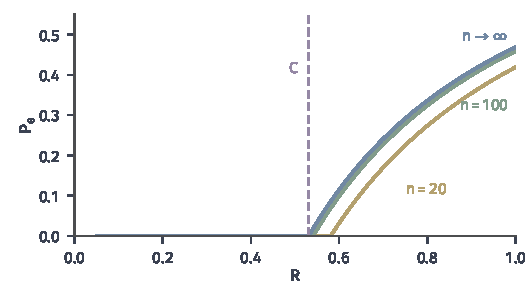
\includegraphics[width=90mm]{figures/07-probability/06-channel-coding/matplotlib/dcc-fano-bound/figure.pdf}
 \caption{翻转概率$0.1$的二元对称信道上，任何$M\geq2^{nR}$的码的平均错误概率下界$1-C/R-1/(nR)$（负值截为零），作为码率$R$的函数：黄线$n=20$，绿线$n=100$，蓝线为$n\to\infty$的极限$1-C/R$；紫色虚线为容量$C=0.531$。}
 \label{fig:dcc-fano-bound}
\end{BookInlineFigure}

证明在两个地方用到了模型假设。数据处理的第二步需要“给定码字后输出与消息无关”，有反馈时编码器的后续输入依赖此前的输出，这一步要重新论证。引理~\ref{lem:dcc-block-bound}需要无记忆。另外，下界$1-C/R$只说错误不能趋于零，并没有说错误趋于$1$。离散无记忆信道上，码率高于容量时错误概率实际上趋于$1$，这称为强逆定理；证明要控制信息密度的集中程度，而不只是它的均值，篇幅较长，可查阅~\scite{math-cover2006information}。

\subsection{最大错误概率}
\label{sec:dcc-max-error}

可达性证明控制的是平均错误概率：大多数消息很少出错，但可能有少数消息出错很多。如果消息不是均匀出现的，例如第~\ref{chap:channel-codes}章把压缩后的索引送进信道时，平均错误小并不能保证实际错误小。需要的是每条消息都可靠，即$\lambda_{\max}$小。

办法是删去坏消息。平均值为$P_{\mathrm{e}}$的一组非负数中，超过平均值两倍的不会多于一半：若超过$2P_{\mathrm{e}}$的有$k\geq1$个，则
\[
 MP_{\mathrm{e}}=\sum_{m}\lambda_m>k\cdot2P_{\mathrm{e}} ,
\]
所以$k<M/2$。这是第~\ref{chap:tail-probabilities}章Markov不等式在均匀分布上的形式。

\begin{lemma}[删去坏码字]
\label{lem:dcc-expurgation}
设$(M,n)$码的平均错误概率为$P_{\mathrm{e}}$，$M\geq2$。则可以从中保留至少$\lceil M/2\rceil$条消息，得到一个最大错误概率不超过$2P_{\mathrm{e}}$的码。
\end{lemma}

\begin{proof}
保留$\lambda_m\leq2P_{\mathrm{e}}$的消息，由上面的计数，保留的个数至少为$\lceil M/2\rceil$。码字不变；解码器把原来判给被删消息的输出块任意改判给一条保留的消息。对保留的消息$m$，判为$m$的输出块只增不减，所以它的条件错误概率不超过原来的$\lambda_m\leq2P_{\mathrm{e}}$。
\end{proof}

这一步称为\term{码字删除}（expurgation）。码率的损失是
\[
 \frac{\log_2M}{n}-\frac{\log_2\lceil M/2\rceil}{n}\leq\frac1n ,
\]
随块长趋于零。所以对$R<C$，先取$R<R'<C$，用可达性得到$M_n\geq2^{nR'}$、平均错误趋于零的码列，再删去一半消息，得到$\lceil M_n/2\rceil\geq2^{nR'-1}\geq2^{nR}$（$n$足够大时）且$\lambda_{\max}\to0$的码列。这就完成了定理~\ref{thm:dcc-coding-theorem}中关于最大错误概率的部分。反方向，最大错误不小于平均错误，逆定理对最大错误口径同样成立。两种口径给出相同的容量。

图~\ref{fig:dcc-expurgation}是一个具体的例子：随机抽取$16$个长度为$14$的二元码字（码率$\tfrac27$），在翻转概率$0.1$的二元对称信道上用最大似然解码（并列时判给编号较小的消息），对全部$2^{14}$个输出块精确求出每条消息的$\lambda_m$。平均错误概率为$0.069$，最差的消息却达到$0.253$。原因是它与另一个码字只差两位，两者似然相同的输出块按并列规则判给了编号较小的那一条，那一条的错误只有$0.040$。删去这一条消息后，剩余$15$条消息的最大错误概率为$0.127$，不超过$2P_{\mathrm{e}}=0.139$，码率变为$\log_215/14\approx0.279$。

\begin{BookInlineFigure}
 \centering
 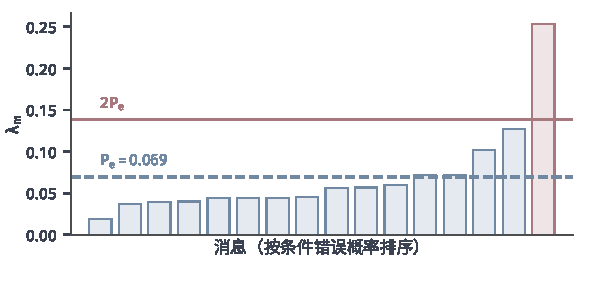
\includegraphics[width=100mm]{figures/07-probability/06-channel-coding/matplotlib/dcc-expurgation/figure.pdf}
 \caption{一个随机二元码（$16$个码字，长度$14$，随机种子$1$）在翻转概率$0.1$的二元对称信道上用最大似然解码时，各消息的条件错误概率$\lambda_m$，按大小排序，均为精确值。蓝色虚线为平均错误概率$0.069$，红线为其两倍；红色柱是被删去的消息。}
 \label{fig:dcc-expurgation}
\end{BookInlineFigure}

删除只在渐近意义下“免费”：$1/n$比特的损失随块长消失，但在有限块长下它是真实的代价。对短码，设计时直接控制每条消息的错误，比事后删除更合适。


\section{二元信道的容量}
\label{sec:dcc-binary}

翻转与擦除是二元输入上最基本的两种损坏。它们的容量各是多少？损坏的概率相同时，哪一种更伤害传输？两个信道都有一个对称性：把输入的$0$与$1$互换，同时把输出的$0$与$1$互换（擦除符号不动），转移矩阵不变。

对称性给出最优输入的候选。若$q$是最优输入分布，把它的两个分量互换得到$\tilde{q}$，由于信道在互换下不变，$I(\tilde{q})=I(q)=C$。由定理~\ref{thm:dcc-capacity-exists}，最优输入组成凸集，所以$\tfrac12q+\tfrac12\tilde{q}=(\tfrac12,\tfrac12)$也最优。于是两个信道的容量都在均匀输入处取到。下面直接算出这个值，再用上界~\eqref{eq:dcc-upper-bound}独立核验。

\subsection{二元对称信道}
\label{sec:dcc-bsc}

设翻转概率为$p\in[0,1]$。给定任一输入，输出是“翻”或“不翻”的二选一，概率为$p$与$1-p$，条件熵是二元熵$h_2(p)$，与输入分布无关：
\[
 H(Y\mid X)=\sum_xq(x)H(W_x)=h_2(p) .
\]
所以互信息只通过输出熵依赖输入分布：
\[
 I(q)=H(Y)-h_2(p)\leq1-h_2(p) ,
\]
因为$Y$只取两个值，$H(Y)\leq1$。均匀输入时，$p_q(1)=\tfrac12(1-p)+\tfrac12p=\tfrac12$，输出均匀，$H(Y)=1$，等号成立。于是
\begin{equation}
 C_{\mathrm{BSC}}(p)=1-h_2(p) .
 \label{eq:dcc-bsc-capacity}
\end{equation}

用式~\eqref{eq:dcc-upper-bound}核验：取$r=(\tfrac12,\tfrac12)$，两行到$r$的散度相同，
\[
 D_{\mathrm{KL}}(W_0\Vert r)=(1-p)\log_2\bigl(2(1-p)\bigr)+p\log_2(2p)=1-h_2(p) ,
\]
$W_1$的计算只是交换两项。所以$C\leq1-h_2(p)$，而均匀输入达到这个值。这一核验不依赖对称性论证，也说明条件~\eqref{eq:dcc-kkt}在均匀输入处成立。

$p=0.1$时，
\[
 h_2(0.1)=0.1\log_210+0.9\log_2\tfrac{10}{9}\approx0.469 ,
\]
容量约为$0.531$比特每次使用。三次重复码以码率$\tfrac13$达到$0.028$的错误；编码定理说，用足够长的码，码率可以接近$0.531$而错误仍趋于零。

\paragraph{端点}
$p=0$时信道无噪声，$C=1$。$p=\tfrac12$时输出与输入独立，无论发什么，接收端看到的都是公平硬币，$C=0$。$p=1$时每个符号都被翻转，但翻转是确定的，接收端把收到的符号全部取反就能完全恢复，$C=1-h_2(1)=1$。所以“翻转发生”与“信息损失”不是一回事：损失来自不知道哪些符号被翻转，即翻转的不可预测性。$h_2(p)$关于$p=\tfrac12$对称，翻转概率$0.9$与$0.1$的信道容量相同。

\subsection{二元擦除信道}
\label{sec:dcc-bec}

设擦除概率为$\varepsilon\in[0,1]$，输出取$0$、$\mathrm{e}$、$1$。这里换一个分解更方便：$I(X;Y)=H(X)-H(X\mid Y)$，计算接收端看到输出后对输入还剩多少不确定性。

看到$0$或$1$时，输入就是这个值，没有剩余的不确定性。看到$\mathrm{e}$时，因为擦除与输入无关，
\[
 \mathbb{P}(X=x\mid Y=\mathrm{e})=\frac{q(x)\varepsilon}{\varepsilon}=q(x) ,
\]
输入仍是原来的分布，剩余$H(X)$。$Y=\mathrm{e}$的概率是$\varepsilon$，所以$H(X\mid Y)=\varepsilon H(X)$，并且
\[
 I(q)=(1-\varepsilon)H(X)\leq1-\varepsilon .
\]
均匀输入使$H(X)=1$，等号成立：
\begin{equation}
 C_{\mathrm{BEC}}(\varepsilon)=1-\varepsilon .
 \label{eq:dcc-bec-capacity}
\end{equation}
这个结果有直接的读法：平均有比例$1-\varepsilon$的符号原样到达，每个携带一比特，被擦除的符号什么也不携带。

核验上界：均匀输入的输出分布是
\[
 r=\Bigl(\frac{1-\varepsilon}2,\ \varepsilon,\ \frac{1-\varepsilon}2\Bigr) ,
\]
第一行到它的散度为
\[
 D_{\mathrm{KL}}(W_0\Vert r)=(1-\varepsilon)\log_2\frac{1-\varepsilon}{(1-\varepsilon)/2}+\varepsilon\log_2\frac{\varepsilon}{\varepsilon}=1-\varepsilon ,
\]
第二行相同（$0<\varepsilon<1$；$\varepsilon=1$时两行都是集中在$\mathrm{e}$上的分布，散度为$0$）。由式~\eqref{eq:dcc-upper-bound}，$C\leq1-\varepsilon$。端点$\varepsilon=0$给出无噪声信道的$1$，$\varepsilon=1$时什么也收不到，容量为$0$。

\paragraph{已知错误位置的价值}
比较损坏概率相同的两个信道。图~\ref{fig:dcc-flip-vs-erasure}把同一个输入块分别送进两个信道，在同样两个位置发生损坏。擦除信道的接收端看到$\mathrm{e}$，确切知道哪里缺了信息，其余位置完全可信；对称信道的接收端看到的是普通的$0$和$1$，不知道哪两位是错的，每一位都只能部分相信。

\begin{BookInlineFigure}
 \centering
 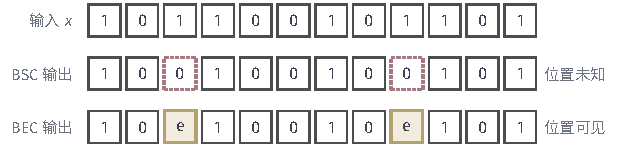
\includegraphics[width=104.5mm]{figures/07-probability/06-channel-coding/tikz/dcc-flip-vs-erasure/figure.pdf}
 \caption{同一个$12$位输入块在第$3$、$9$位受到损坏。二元对称信道把这两位翻转，结果看起来与其他位无异，红色虚线框只是标给读者看的；二元擦除信道把这两位变成可见的擦除符号$\mathrm{e}$（黄色）。}
 \label{fig:dcc-flip-vs-erasure}
\end{BookInlineFigure}

图~\ref{fig:dcc-capacity-curves}比较两条容量曲线。损坏概率都是$0.1$时，擦除信道的容量是$0.9$，对称信道只有$0.531$。差值$h_2(p)-p$可以理解为找出错误位置的代价：在$n$个符号中指出约$np$个翻转位置，需要约$nh_2(p)$比特的描述，而擦除信道把这些位置免费告诉了接收端，只损失被擦掉的$np$比特本身。对$0<p<\tfrac12$总有$h_2(p)>p$，所以未知的翻转总比可见的擦除更伤害传输。

\begin{BookInlineFigure}
 \centering
 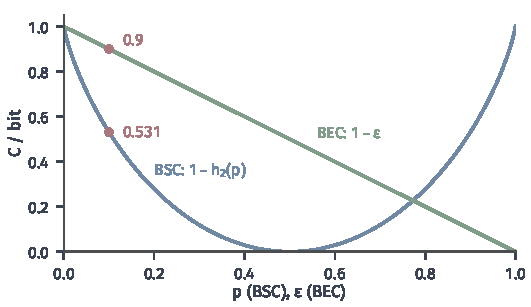
\includegraphics[width=90mm]{figures/07-probability/06-channel-coding/matplotlib/dcc-capacity-curves/figure.pdf}
 \caption{二元对称信道的容量$1-h_2(p)$（蓝）与二元擦除信道的容量$1-\varepsilon$（绿），横轴为翻转概率或擦除概率。红点标出损坏概率$0.1$时的两个容量$0.531$与$0.9$。蓝线关于$p=\tfrac12$对称：确定的翻转不损失信息。}
 \label{fig:dcc-capacity-curves}
\end{BookInlineFigure}

\paragraph{对称性的作用}
两个信道的均匀输入最优，依赖的是交换$0$与$1$的对称性，不是二元输入本身。第~\ref{sec:dcc-capacity-formula}节的Z信道同样是二元输入，却没有这种对称性：输入$1$会出错而输入$0$不会，最优输入是$q=0.4$，均匀输入少得约$0.011$比特。对一般的转移矩阵，最优输入要从条件~\eqref{eq:dcc-kkt}解出，通常没有闭式，这就需要第~\ref{sec:dcc-numerical}节的数值方法。


\section{输入成本约束}
\label{sec:dcc-costs}

实际发送时，不同符号的代价往往不同。在Z信道中，可以把输入$1$想成发出一个脉冲、输入$0$想成保持静默：脉冲消耗能量，静默不消耗。若能量有限，就不能随意多发$1$。预算会怎样限制传输速率？

给每个输入符号指定一个有限的非负成本$c(x)$，记最小成本$c_{\min}=\min_xc(x)$。设定预算$\Gamma\geq c_{\min}$，要求每一条码字都满足
\begin{equation}
 \sum_{i=1}^{n}c\bigl(x_i(m)\bigr)\leq n\Gamma,\qquad m=1,\dots,M .
 \label{eq:dcc-codeword-budget}
\end{equation}
这里的平均是沿同一条码字的$n$次使用求平均：每次传输一条消息都要守住预算。它不允许一部分消息超支、另一部分消息节省来互相抵消。在预算$\Gamma$下的可达速率按定义~\ref{def:dcc-achievable}定义，只是要求码列中的每个码都满足式~\eqref{eq:dcc-codeword-budget}。本节的例子是Z信道，取$c(0)=0$、$c(1)=1$，于是预算$\Gamma=0.25$意味着每条码字中$1$的个数不超过$n/4$。

\subsection{成本约束下的容量}
\label{sec:dcc-cost-capacity}

无约束时容量是互信息在整个单纯形上的最大值。有预算时，自然的猜测是只在“平均成本不超过预算”的输入分布上取最大值。

\begin{definition}[容量—成本函数]
\label{def:dcc-capacity-cost}
对$\Gamma\geq c_{\min}$，定义
\begin{equation}
 C(\Gamma)=\max\Bigl\{I(q):q\in\Delta_{\mathcal{X}},\ \sum_{x}q(x)c(x)\leq\Gamma\Bigr\} ,
 \label{eq:dcc-capacity-cost}
\end{equation}
称为\term{容量—成本函数}（capacity-cost function）。
\end{definition}

可行集合非空：集中在某个最小成本符号上的分布满足约束。下面的定理列出$C(\Gamma)$的基本性质。

\begin{theorem}[容量—成本函数的性质]
\label{thm:dcc-capacity-cost}
在$[c_{\min},\infty)$上，式~\eqref{eq:dcc-capacity-cost}的最大值存在；$C(\Gamma)$单调不减、是凹函数，在$(c_{\min},\infty)$上连续，并且$C(\Gamma)\leq C$；若某个无约束最优输入的平均成本为$\Gamma^{*}$，则$\Gamma\geq\Gamma^{*}$时$C(\Gamma)=C$。
\end{theorem}

\begin{proof}
可行集合是单纯形与一个闭半空间的交，非空且有界闭，$I$连续，所以最大值存在。预算增大时可行集合变大，最大值不减；它总是整个单纯形的子集，所以$C(\Gamma)\leq C$；$\Gamma\geq\Gamma^{*}$时可行集合包含无约束最优输入，所以取到$C$。

凹性。取预算$\Gamma_1,\Gamma_2$及相应的最优输入$q_1,q_2$，$\theta\in[0,1]$。混合$q_\theta=\theta q_1+(1-\theta)q_2$的平均成本是$\theta\Gamma_1+(1-\theta)\Gamma_2$以下，所以在该预算下可行；由$I$的凹性，
\[
 C\bigl(\theta\Gamma_1+(1-\theta)\Gamma_2\bigr)\geq I(q_\theta)\geq\theta C(\Gamma_1)+(1-\theta)C(\Gamma_2) .
\]
有限的凹函数在开区间内部连续，所以$C$在$(c_{\min},\infty)$上连续。
\end{proof}

在端点$c_{\min}$处，$C$未必右连续。凹性说明预算越多，每多一单位预算带来的容量增量越小，直到达到$\Gamma^{*}$后增量为零。

\paragraph{Z信道的例子}
平均成本是$\sum_xq(x)c(x)=q$，约束就是$q\leq\Gamma$。由第~\ref{sec:dcc-capacity-formula}节，$I(q)=h_2(q/2)-q$在$[0,0.4]$上递增、在$0.4$处达到最大值。所以
\[
 C(\Gamma)=h_2\Bigl(\frac\Gamma2\Bigr)-\Gamma\quad(0\leq\Gamma\leq0.4),\qquad C(\Gamma)=\log_2\frac54\quad(\Gamma\geq0.4) .
\]
预算$\Gamma=0.25$时，最优输入为$q=0.25$，
\[
 C(0.25)=h_2(0.125)-0.25\approx0.5436-0.25=0.2936 ,
\]
比无约束容量$0.3219$少约$0.028$比特。图~\ref{fig:dcc-cost-capacity}(a)画出可行的输入范围，(b)画出整条$C(\Gamma)$曲线：它先凹地上升，在$\Gamma=0.4$之后变平。

\begin{BookInlineFigure}
 \centering
 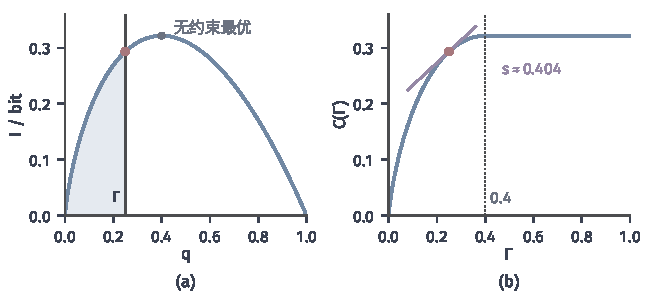
\includegraphics[width=110mm]{figures/07-probability/06-channel-coding/matplotlib/dcc-cost-capacity/figure.pdf}
 \caption{Z信道在成本$c(0)=0$、$c(1)=1$下的容量—成本函数。(a) 互信息$I(q)=h_2(q/2)-q$，浅蓝区域是预算$\Gamma=0.25$允许的输入$q\leq\Gamma$，红点为约束下的最优点，灰点为无约束最优点$q=0.4$；(b) $C(\Gamma)$，紫线是$\Gamma=0.25$处的切线，斜率$s\approx0.404$比特每单位成本，点线标出$\Gamma=0.4$。}
 \label{fig:dcc-cost-capacity}
\end{BookInlineFigure}

\paragraph{Lagrange乘子：预算的边际价值}
图~\ref{fig:dcc-cost-capacity}(b)中切线的斜率回答“再多给一单位预算，容量能增加多少”。把约束用乘子$s\geq0$并入目标，考虑
\begin{equation}
 \max_{q\in\Delta_{\mathcal{X}}}\Bigl[I(q)-s\sum_xq(x)c(x)\Bigr]+s\Gamma .
 \label{eq:dcc-lagrangian}
\end{equation}
对每个$s\geq0$与每个可行的$q$，被减去的$s(\sum_xq(x)c(x)-\Gamma)$非正，所以$I(q)$不超过式~\eqref{eq:dcc-lagrangian}；对可行的$q$取最大值，得到
\begin{equation}
 C(\Gamma)\leq\max_{q}\Bigl[I(q)-s\sum_xq(x)c(x)\Bigr]+s\Gamma\qquad\text{对每个}\ s\geq0 .
 \label{eq:dcc-weak-duality}
\end{equation}
这是弱对偶。$\Gamma>c_{\min}$时，集中在最小成本符号上的分布严格满足预算，目标是凹函数，约束是线性的，于是强对偶成立：式~\eqref{eq:dcc-weak-duality}右边对$s$的最小值等于$C(\Gamma)$，达到最小值的$s$是$C$在$\Gamma$处的切线斜率（$C$在该点可微时）。凸优化对偶的一般理论可参考\BookChapterRef{chap:duality}{卷五第18章“对偶问题”}。

固定$s$后，式~\eqref{eq:dcc-lagrangian}中的最大化与定理~\ref{thm:dcc-kkt}的问题相同，只是线性项多了$-s\sum_xq(x)c(x)$。在定理~\ref{thm:dcc-kkt}必要性的求导中，这一项沿$q_t=(1-t)q^{*}+t\delta_{x'}$的右导数是$-s\bigl(c(x')-\sum_xq^{*}(x)c(x)\bigr)$，充分性部分的上界也照样成立。所以最优条件变为：存在常数$c'$，使
\begin{equation}
 \begin{aligned}
 D_{\mathrm{KL}}(W_x\Vert p^{*})-s\,c(x)&=c'\quad\text{若}\ q^{*}(x)>0 ,\\
 D_{\mathrm{KL}}(W_x\Vert p^{*})-s\,c(x)&\leq c'\quad\text{若}\ q^{*}(x)=0 .
 \end{aligned}
 \label{eq:dcc-kkt-cost}
\end{equation}
读法是：每个输入的信息贡献扣去它按“影子价格”$s$折算的成本后，被使用的输入应当一样划算。

在Z信道$\Gamma=0.25$处核验。斜率为
\[
 s=I'(0.25)=\frac12\log_2\frac{2-0.25}{0.25}-1=\frac12\log_27-1\approx0.4037 .
\]
输出分布$p^{*}=(\tfrac78,\tfrac18)$，两行的散度为
\[
 \begin{aligned}
 D_{\mathrm{KL}}(W_0\Vert p^{*})&=\log_2\frac87\approx0.1926 ,\\
 D_{\mathrm{KL}}(W_1\Vert p^{*})&=\frac12\log_2\frac47+\frac12\log_24=\frac12\log_2\frac{16}7\approx0.5963 .
 \end{aligned}
\]
扣去成本后，$0.1926-0=0.1926$，$0.5963-0.4037=0.1926$，两者相等；并且$C(\Gamma)-s\Gamma=0.2936-0.1009=0.1927$，与舍入误差内一致。精确地，
\[
 \frac12\log_2\frac{16}7-\Bigl(\frac12\log_27-1\Bigr)=3-\log_27=\log_2\frac87 .
\]

\paragraph{期望约束与逐条预算}
式~\eqref{eq:dcc-capacity-cost}约束的是输入分布的期望成本，它是对单个随机符号的设计要求；式~\eqref{eq:dcc-codeword-budget}约束的是每一条具体码字的成本总和。按期望成本恰为$\Gamma$的分布独立抽取码字，大约一半码字会超出预算。两者之间的联系需要论证，这是下一小节的内容。

\subsection{满足预算的编码}
\label{sec:dcc-cost-coding}

下面的定理说明，在逐条预算下，$C(\Gamma)$正是可靠传输的速率极限。

\begin{theorem}[成本约束下的编码定理]
\label{thm:dcc-cost-coding}
设$\Gamma>c_{\min}$。在每条码字满足式~\eqref{eq:dcc-codeword-budget}的要求下，每个$R<C(\Gamma)$都可达，并且可以要求最大错误概率趋于零；每个$R>C(\Gamma)$都不可达。
\end{theorem}

\begin{proof}
可达性。设$R<C(\Gamma)$。由定理~\ref{thm:dcc-capacity-cost}，$C$在$\Gamma$处连续，可以取$\Gamma'\in(c_{\min},\Gamma)$使$C(\Gamma')>R$。取$q'$使$\sum_xq'(x)c(x)\leq\Gamma'$且$I(q')=C(\Gamma')$。这一步为预算留出了余量$\Gamma-\Gamma'>0$。

按$q'$抽取随机码本，用联合典型解码。定理~\ref{thm:dcc-achievability}的证明对任何满足$I(q)>R$的输入分布都成立，所以存在$\delta_n\to0$，使每条消息的期望错误$\mathbb{E}[\lambda_m]\leq\delta_n$。另一方面，记$B_m$为第$m$条码字超出预算的事件。码字的平均成本$\frac1n\sum_ic(\mathsf{X}_i(m))$是$n$个独立同分布、取值有界的变量的平均，均值不超过$\Gamma'<\Gamma$，由弱大数律，
\[
 \beta_n=\mathbb{P}(B_m)\leq\mathbb{P}\Bigl(\frac1n\sum_{i=1}^{n}c(\mathsf{X}_i(m))-\Gamma'>\Gamma-\Gamma'\Bigr)\to0 .
\]
于是随机码本满足
\[
 \mathbb{E}\Bigl[P_{\mathrm{e}}+\frac1M\sum_{m=1}^{M}\mathbf{1}_{B_m}\Bigr]\leq\delta_n+\beta_n=:\eta_n ,
\]
存在一个具体码本，其平均错误概率与超支码字的比例之和不超过$\eta_n$。

删去两类消息：条件错误概率超过$4\eta_n$的消息，按第~\ref{sec:dcc-max-error}小节的计数少于$M/4$条；超支的消息，至多$\eta_nM$条，$n$足够大使$\eta_n\leq\tfrac14$时不超过$M/4$条。保留的消息至少有$M/2$条，每条码字都守住预算，最大错误概率不超过$4\eta_n$，码率损失不超过$1/n$。与引理~\ref{lem:dcc-expurgation}后的论证一样，先用$R<R'<C(\Gamma)$构造码列再删除，就得到码率不低于$R$的码列。

逆定理。设一列满足逐条预算的码有$M\geq2^{nR}$且$P_{\mathrm{e}}\to0$。消息均匀，记第$i$个输入符号$X_i$的分布为$q_i$，期望成本$\Gamma_i=\mathbb{E}[c(X_i)]$。逆定理证明中的Fano与数据处理步骤不变，引理~\ref{lem:dcc-block-bound}的第一个不等式给出
\[
 \log_2M\leq1+P_{\mathrm{e}}\log_2M+\sum_{i=1}^{n}I(X_i;Y_i)\leq1+P_{\mathrm{e}}\log_2M+\sum_{i=1}^{n}C(\Gamma_i) .
\]
由$C$的凹性（Jensen不等式）与单调性，
\[
 \frac1n\sum_{i=1}^{n}C(\Gamma_i)\leq C\Bigl(\frac1n\sum_{i=1}^{n}\Gamma_i\Bigr)\leq C(\Gamma) ,
\]
最后一步因为
\[
 \frac1n\sum_{i=1}^{n}\Gamma_i=\mathbb{E}\Bigl[\frac1n\sum_{i=1}^{n}c(X_i)\Bigr]\leq\Gamma :
\]
每条码字的平均成本都不超过$\Gamma$，对消息平均后也不超过。于是$P_{\mathrm{e}}\geq1-(nC(\Gamma)+1)/\log_2M$，与定理~\ref{thm:dcc-converse}同理，$R>C(\Gamma)$不可达。
\end{proof}

可达性证明中的两个余量各有作用。码率余量$C(\Gamma')-R>0$控制解码错误，与无约束时相同；预算余量$\Gamma-\Gamma'>0$让大数律把码字成本压在预算以内。若直接用期望成本恰为$\Gamma$的分布，超支的码字比例不趋于零，删除会损失一个固定比例的消息。图~\ref{fig:dcc-codeword-cost}画出Z信道上$q'=0.22$、$\Gamma=0.25$时单条随机码字的平均成本分布：$n=50$时超支的概率约为$0.296$，$n=400$时降到约$0.067$，并继续趋于零。所用输入的互信息为$C(0.22)=h_2(0.11)-0.22\approx0.280$，略低于$C(0.25)=0.294$，这是为预算余量付出的码率。

\begin{BookInlineFigure}
 \centering
 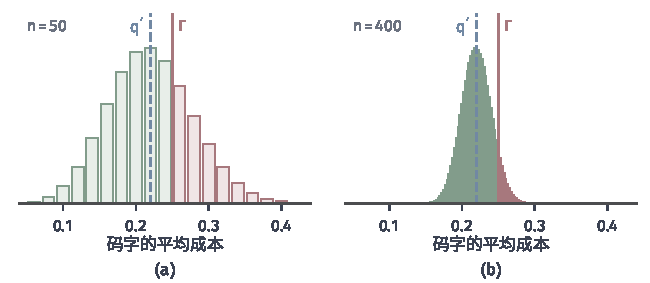
\includegraphics[width=110mm]{figures/07-probability/06-channel-coding/matplotlib/dcc-codeword-cost/figure.pdf}
 \caption{Z信道、成本$c(1)=1$，码字符号独立地以概率$q'=0.22$取$1$时，单条码字的平均成本$K/n$（$K\sim\mathrm{Bin}(n,0.22)$）的精确分布。蓝色虚线为$q'$，红线为预算$\Gamma=0.25$，红色柱为超出预算的码字。(a) $n=50$；(b) $n=400$。}
 \label{fig:dcc-codeword-cost}
\end{BookInlineFigure}

逆定理只用到了“对消息平均的成本不超过$\Gamma$”。所以即使放宽要求，只限制各码字成本的平均值，容量也不会超过$C(\Gamma)$；而可达性给出的码满足更严格的逐条预算。两种口径给出同一个容量。

\paragraph{预算等于最小成本}
$\Gamma=c_{\min}$时，余量论证无法进行，因为不存在$\Gamma'<\Gamma$。但此时约束本身变得简单：每个$c(x_i)\geq c_{\min}$，总和不超过$nc_{\min}$只能让每一项都等于$c_{\min}$。所以码字只能使用集合$\mathcal{X}_0=\{x:c(x)=c_{\min}\}$中的符号，成本约束自动满足。这相当于把输入字母表缩小为$\mathcal{X}_0$、转移矩阵只保留相应的行，对这个新信道应用无约束的定理~\ref{thm:dcc-coding-theorem}，容量为$\max\{I(q):q\ \text{支撑在}\ \mathcal{X}_0\ \text{上}\}$。这恰好等于$C(c_{\min})$，因为平均成本等于$c_{\min}$的分布正是支撑在$\mathcal{X}_0$上的分布。在Z信道中$\mathcal{X}_0=\{0\}$，只能发送$0$，容量为零。


\section{容量的数值计算}
\label{sec:dcc-numerical}

对称信道和Z信道的容量都能手算，一般的转移矩阵却不行：条件~\eqref{eq:dcc-kkt}是关于$q$的非线性方程组，还带着“哪些输入概率为零”的组合选择。互信息是单纯形上的凹函数，原则上任何凸优化方法都能求最大值；但这个问题有特殊结构，可以得到每步都有闭式、自动留在单纯形内、并且随时给出容量上下界的迭代。它称为\term{Blahut–Arimoto算法}（Blahut–Arimoto algorithm）。

\paragraph{主要思想}
出发点是式~\eqref{eq:dcc-mi-divergence}：互信息是各输入的信息贡献$D_{\mathrm{KL}}(W_x\Vert p_q)$按$q$的平均。若某个输入的贡献高于平均，就应当多用它。Blahut–Arimoto算法把这个直觉做成乘性的重新加权，下面从一个双变量的目标推出它。

引入一个“反向”的条件分布$r(x\mid y)$：对每个$y$，$r(\cdot\mid y)$是$\mathcal{X}$上的概率分布，它表示接收端看到$y$后对输入的猜测。定义
\[
 J(q,r)=\sum_{x,y}q(x)W(y\mid x)\log_2\frac{r(x\mid y)}{q(x)} .
\]
固定$q$时，最好的猜测是真实的后验$r_q(x\mid y)=q(x)W(y\mid x)/p_q(y)$。因为$r_q(x\mid y)/q(x)=W(y\mid x)/p_q(y)$，所以$J(q,r_q)=I(q)$；而对任意$r$，
\[
 \begin{aligned}
 I(q)-J(q,r)&=\sum_{x,y}q(x)W(y\mid x)\log_2\frac{r_q(x\mid y)}{r(x\mid y)}\\
 &=\sum_yp_q(y)\,D_{\mathrm{KL}}\bigl(r_q(\cdot\mid y)\Vert r(\cdot\mid y)\bigr)\geq0 .
 \end{aligned}
\]
于是$I(q)=\max_rJ(q,r)$，容量可以写成两个变量的联合最大值
\begin{equation}
 C=\max_{q}\max_{r}J(q,r) .
 \label{eq:dcc-ba-double-max}
\end{equation}

反过来固定$r$，对$q$最大化。记$a(x)=\sum_yW(y\mid x)\log_2r(x\mid y)$，目标是$\sum_xq(x)\bigl(a(x)-\log_2q(x)\bigr)$。令$\tilde{q}(x)=2^{a(x)}/Z$，$Z=\sum_x2^{a(x)}$，则
\[
 \sum_xq(x)\bigl(a(x)-\log_2q(x)\bigr)=\log_2Z-D_{\mathrm{KL}}(q\Vert\tilde{q}) ,
\]
所以最大值点是$q=\tilde{q}$，最大值是$\log_2Z$。

两步交替进行：由$q_t$取后验$r_{q_t}$，再由它算出新的$q_{t+1}$。代入后验，
\[
 a(x)=\log_2q_t(x)+\sum_{y}W(y\mid x)\log_2\frac{W(y\mid x)}{p_{q_t}(y)} ,
\]
后一项正是第$x$行的散度。记
\[
 p_t=p_{q_t},\qquad D_t(x)=D_{\mathrm{KL}}\bigl(W_x\Vert p_t\bigr) ,
\]
得到更新公式
\begin{equation}
 q_{t+1}(x)=\frac{q_t(x)\,2^{D_t(x)}}{\sum_{x'}q_t(x')\,2^{D_t(x')}} .
 \label{eq:dcc-ba-update}
\end{equation}
贡献$D_t(x)$大的输入按指数放大，小的相对缩小，与开头的直觉一致。不动点处，凡是$q(x)>0$的输入，$2^{D(x)}$必须等于归一化常数，即散度相等，这正是条件~\eqref{eq:dcc-kkt}。

每一轮还能顺带得到容量的上下界。下界：$\log_2\sum_xq_t(x)2^{D_t(x)}$是$J(q_{t+1},r_{q_t})$，不超过$I(q_{t+1})$，更不超过$C$。上界：在式~\eqref{eq:dcc-upper-bound}中取$r=p_t$。于是
\begin{equation}
 L_t=\log_2\sum_xq_t(x)\,2^{D_t(x)}\ \leq\ C\ \leq\ U_t=\max_xD_t(x) .
 \label{eq:dcc-ba-bounds}
\end{equation}
两个界都是严格成立的不等式，不是估计值；$U_t-L_t$就是当前对容量的误差保证。交替对两个变量分别取最大的做法，是卷五分块坐标方法的一个特例，可参考\BookChapterRef{chap:block-optimization}{卷五第12章“分块优化”}。第~\ref{chap:rate-distortion}章计算率失真函数时用的是同一结构，只是那里最小化，并带有失真的指数权重。

\paragraph{计算过程}
下面以Z信道为例走一遍，转移矩阵的两行是$W_0=(1,0)$与$W_1=(\tfrac12,\tfrac12)$。

\needspace{6\baselineskip}
\paragraph{变量}
\begin{itemize}
 \item $q_t$：长度为$\lvert\mathcal{X}\rvert$的概率向量，第$t$轮的输入分布；
 \item $p_t$：长度为$\lvert\mathcal{Y}\rvert$的概率向量，$p_t=q_t\bm{W}$；
 \item $D_t$：长度为$\lvert\mathcal{X}\rvert$的向量，$D_t(x)=D_{\mathrm{KL}}(W_x\Vert p_t)$；
 \item $L_t,U_t$：容量的下界与上界；$\tau>0$：要求的精度。
\end{itemize}

\paragraph{初始化}
取支撑为整个$\mathcal{X}$的初始分布，通常取均匀分布$q_0(x)=1/\lvert\mathcal{X}\rvert$。例中$q_0=(\tfrac12,\tfrac12)$，$\tau=0.01$。

\needspace{6\baselineskip}
\paragraph{每轮更新}
对$t=0,1,2,\dots$依次执行：
\begin{enumerate}
 \item 输出分布：$p_t=q_t\bm{W}$。例中第$0$轮，
 \[
  p_0=\tfrac12(1,0)+\tfrac12(\tfrac12,\tfrac12)=(\tfrac34,\tfrac14) .
 \]

 \item 各行散度：按$D_t(x)=D_{\mathrm{KL}}(W_x\Vert p_t)$计算，$W(y\mid x)=0$的项记为零。例中
 \[
  \begin{aligned}
  D_0(0)&=\log_2\frac43\approx0.4150 ,\\
  D_0(1)&=\frac12\log_2\frac{1/2}{3/4}+\frac12\log_2\frac{1/2}{1/4}=\frac12\log_2\frac43\approx0.2075 .
  \end{aligned}
 \]

 \item 上下界：由式~\eqref{eq:dcc-ba-bounds}计算。例中$2^{D_0(0)}=\tfrac43$，$2^{D_0(1)}=\tfrac{2}{\sqrt3}\approx1.1547$，
 \[
  L_0=\log_2\Bigl(\tfrac12\cdot\tfrac43+\tfrac12\cdot1.1547\Bigr)=\log_21.2440\approx0.3150 ,
 \]
 \[
  U_0=\max\{0.4150,\ 0.2075\}=0.4150 .
 \]
 若$U_t-L_t\leq\tau$，停止。例中差距为$0.1000$，继续。

 \item 重新加权：由式~\eqref{eq:dcc-ba-update}，
 \[
  q_1=\frac{(0.6667,\ 0.5774)}{1.2440}=(0.5359,\ 0.4641) .
 \]
 精确值是$q_1(1)=2\sqrt3-3$。输入$1$的贡献低于平均，它的概率下降了。
\end{enumerate}

例中第$1$轮的四步依次得到
\[
 p_1=(0.7679,\ 0.2321),\qquad D_1=(0.3809,\ 0.2442) ,
\]
\[
 L_1=\log_2(0.5359\times1.3021+0.4641\times1.1844)\approx0.3191,\qquad U_1\approx0.3809 ,
\]
差距为$0.0618$，更新得$q_2=(0.5594,0.4406)$。各轮结果如下表。

\begin{BookInlineTable}
 \centering
 \caption{Z信道上Blahut–Arimoto迭代的各轮数值，$q_0=(\tfrac12,\tfrac12)$，容量真值为$\log_2(5/4)\approx0.32193$。}
 \label{tab:dcc-ba-rounds}
 \begin{tabular}{cccccc}
  \toprule
  $t$ & $q_t(1)$ & $D_t(0)$ & $D_t(1)$ & $L_t$ & $U_t$ \\
  \midrule
  $0$ & $0.50000$ & $0.41504$ & $0.20752$ & $0.31501$ & $0.41504$ \\
  $1$ & $0.46410$ & $0.38092$ & $0.24420$ & $0.31907$ & $0.38092$ \\
  $2$ & $0.44063$ & $0.35904$ & $0.27070$ & $0.32078$ & $0.35904$ \\
  $3$ & $0.42560$ & $0.34520$ & $0.28882$ & $0.32147$ & $0.34520$ \\
  $4$ & $0.41607$ & $0.33649$ & $0.30079$ & $0.32175$ & $0.33649$ \\
  $5$ & $0.41007$ & $0.33104$ & $0.30854$ & $0.32186$ & $0.33104$ \\
  \bottomrule
 \end{tabular}
\end{BookInlineTable}

第$5$轮差距$U_5-L_5=0.0092\leq0.01$，停止。最终得到容量的保证区间与近似最优输入
\[
 0.32186\leq C\leq0.33104,\qquad q_5\approx(0.590,\ 0.410) .
\]
真值$0.32193$确实在区间内，最优输入是$(0.6,0.4)$。图~\ref{fig:dcc-ba-z}画出更多轮次：$q_t(1)$单调地趋向$0.4$；下界几乎一开始就贴近容量，上界下降较慢，差距主要由上界决定。

\begin{BookInlineFigure}
 \centering
 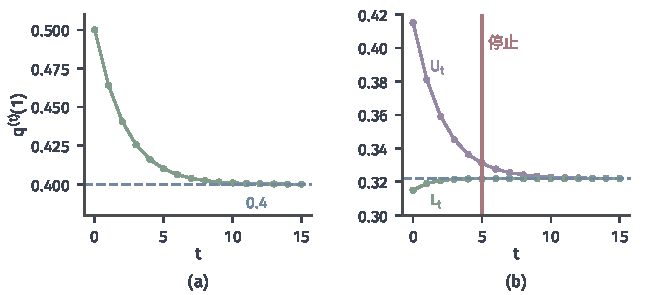
\includegraphics[width=110mm]{figures/07-probability/06-channel-coding/matplotlib/dcc-ba-z/figure.pdf}
 \caption{Z信道上从$q_0=(\tfrac12,\tfrac12)$出发的Blahut–Arimoto迭代。(a) 绿点为$q_t(1)$，蓝色虚线为最优值$0.4$；(b) 紫线为上界$U_t$，绿线为下界$L_t$，蓝色虚线为容量$\log_2(5/4)$，红线标出第一次满足$U_t-L_t\leq0.01$的轮次$t=5$。}
 \label{fig:dcc-ba-z}
\end{BookInlineFigure}

\paragraph{收敛性}
下界的收敛可以完整证明，并且给出速度。

\begin{theorem}[Blahut–Arimoto迭代的收敛]
\label{thm:dcc-ba-convergence}
设$q_0$的支撑是整个$\mathcal{X}$，$q^{*}$是任一最优输入分布。则$I(q_t)$与$L_t$都单调不减，并且
\begin{equation}
 C-L_T\leq\frac{D_{\mathrm{KL}}(q^{*}\Vert q_0)}{T+1},\qquad T=0,1,2,\dots .
 \label{eq:dcc-ba-rate}
\end{equation}
$q_0$均匀时右边不超过$\log_2\lvert\mathcal{X}\rvert/(T+1)$。
\end{theorem}

\begin{proof}
单调性。记$r_t=r_{q_t}$。由$J$对两个变量分别取最大的性质，
\[
 \begin{aligned}
 I(q_t)=J(q_t,r_t)&\leq J(q_{t+1},r_t)=L_t\\
 &\leq J(q_{t+1},r_{t+1})=I(q_{t+1})\leq J(q_{t+2},r_{t+1})=L_{t+1} .
 \end{aligned}
\]

速度。更新公式~\eqref{eq:dcc-ba-update}的对数形式是$\log_2\frac{q_{t+1}(x)}{q_t(x)}=D_t(x)-L_t$；$q_0$处处为正，每步乘以正数，所以$q_t$处处为正。按$q^{*}$求平均，
\[
 \sum_xq^{*}(x)\log_2\frac{q_{t+1}(x)}{q_t(x)}=\sum_xq^{*}(x)D_t(x)-L_t .
\]
定理~\ref{thm:dcc-kkt}证明中的恒等式（取$q=q^{*}$、$r=p_t$）给出
\[
 \sum_xq^{*}(x)D_t(x)=C+D_{\mathrm{KL}}(p^{*}\Vert p_t)\geq C ,
\]
所以右边不小于$C-L_t$。对$t=0,\dots,T$求和，左边逐项相消，
\[
 \begin{aligned}
 D_{\mathrm{KL}}(q^{*}\Vert q_0)-D_{\mathrm{KL}}(q^{*}\Vert q_{T+1})&=\sum_{t=0}^{T}\sum_xq^{*}(x)\log_2\frac{q_{t+1}(x)}{q_t(x)}\\
 &\geq\sum_{t=0}^{T}(C-L_t)\geq(T+1)(C-L_T) ,
 \end{aligned}
\]
最后一步用了$L_t$单调不减。$D_{\mathrm{KL}}(q^{*}\Vert q_{T+1})\geq0$，移项即得式~\eqref{eq:dcc-ba-rate}。均匀初始时
\[
 D_{\mathrm{KL}}(q^{*}\Vert q_0)=\log_2\lvert\mathcal{X}\rvert-H(q^{*})\leq\log_2\lvert\mathcal{X}\rvert .
\]
\end{proof}

上界$U_t$同样收敛到$C$，因为$p_t$收敛到唯一的最优输出分布；这一部分的证明更长，可查阅~\scite{math-cover2006information}。实践中不需要它的速度：只要算出$U_t$与$L_t$，区间$[L_t,U_t]$本身就是可验证的结论。

\paragraph{初始支撑与零概率输入}
证明中“$q_0$处处为正”不可省略。若$q_0(x)=0$，乘性更新使$q_t(x)$永远为零，迭代实际是在去掉输入$x$的信道上进行；若$x$是有用的输入，迭代会收敛到一个偏小的值。这时上界会暴露问题：$U_t$对全部输入取最大值，包括概率为零的输入，于是差距$U_t-L_t$不会趋于零。同样的原因，初始支撑完整时$p_t(y)>0$对一切可能出现的输出成立，散度不会出现除以零。

反过来，最优输入可能给某些符号零概率，迭代却只能让它们的概率趋于零而不能到达零。考虑三输入二输出的信道，三行为$(1,0)$、$(0,1)$、$(\tfrac12,\tfrac12)$：前两个输入无噪声，第三个输入的输出与输入无关。容量为$1$比特，最优输入是$(\tfrac12,\tfrac12,0)$。从均匀分布出发，由对称性$p_t=(\tfrac12,\tfrac12)$始终不变，散度始终为$(1,1,0)$，每轮第三个分量相对其余两个缩小一半：
\[
 q_t(2)=\frac{1}{2^{t+1}+1}:\qquad \tfrac13,\ \tfrac15,\ \tfrac19,\ \tfrac1{17},\ \dots
\]
上界从第$0$轮起就等于$1$，下界$L_t=\log_2(2-q_t(2))$的差距按几何速度缩小，远快于式~\eqref{eq:dcc-ba-rate}保证的$\log_23/(t+1)$。图~\ref{fig:dcc-ba-support}画出这两点。

\begin{BookInlineFigure}
 \centering
 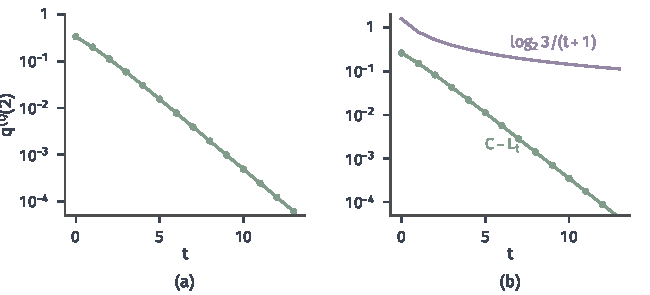
\includegraphics[width=110mm]{figures/07-probability/06-channel-coding/matplotlib/dcc-ba-support/figure.pdf}
 \caption{三行分别为$(1,0)$、$(0,1)$、$(\tfrac12,\tfrac12)$的信道上，从均匀分布出发的Blahut–Arimoto迭代，纵轴均为对数坐标。(a) 无用输入的概率$q_t(2)=1/(2^{t+1}+1)$按几何速度减小，但始终为正；(b) 绿线为下界的差距$C-L_t$，紫线为定理~\ref{thm:dcc-ba-convergence}的保证$\log_23/(t+1)$；上界$U_t$从第$0$轮起就等于$C=1$。}
 \label{fig:dcc-ba-support}
\end{BookInlineFigure}

这个例子说明两件事。第一，概率很小不等于应当为零，不能仅凭$q_t(x)$小就把输入删掉；需要删减时，应先用上下界确认删去后容量不变。第二，迭代变化小也不是停止的依据。Z信道第$7$轮以后$q_t$每轮只变化约$0.002$，差距仍有$0.004$；在收敛更慢的信道上，变化可以极小而离最优仍远。应当用的是$U_t-L_t$。

\paragraph{计算量}
每轮需要算$p_t=q_t\bm{W}$与全部散度，各需要$O(\lvert\mathcal{X}\rvert\lvert\mathcal{Y}\rvert)$次运算，更新与求界只需$O(\lvert\mathcal{X}\rvert)$。由式~\eqref{eq:dcc-ba-rate}，下界达到精度$\tau$至多需要约$\log_2\lvert\mathcal{X}\rvert/\tau$轮；实际中常快得多。

\paragraph{带成本约束的迭代}
对第~\ref{sec:dcc-costs}节的问题，先固定乘子$s\geq0$，求式~\eqref{eq:dcc-lagrangian}中的最大化。推导与上面相同，只是$a(x)$多了一项$-s\,c(x)$，更新变为
\begin{equation}
 q_{t+1}(x)\propto q_t(x)\,2^{D_t(x)-s\,c(x)} .
 \label{eq:dcc-ba-cost-update}
\end{equation}
固定$s$迭代到收敛，得到$C(\Gamma)$曲线上斜率为$s$的点：其横坐标是平均成本$\Gamma(s)=\sum_xq(x)c(x)$，纵坐标是$I(q)$。$s$越大，成本越受惩罚，$\Gamma(s)$越小。要对给定的$\Gamma$求$C(\Gamma)$，就在外层对$s$二分，使$\Gamma(s)$等于$\Gamma$。

图~\ref{fig:dcc-ba-cost}在Z信道上取$s=0,0.1,\dots,1.5$，各迭代$400$轮，得到的点都落在解析曲线$h_2(\Gamma/2)-\Gamma$上；对$\Gamma=0.25$二分得到$s\approx0.4037$，与第~\ref{sec:dcc-cost-capacity}小节算出的切线斜率一致。$s=0$给出无约束的最优点$\Gamma=0.4$。

\begin{BookInlineFigure}
 \centering
 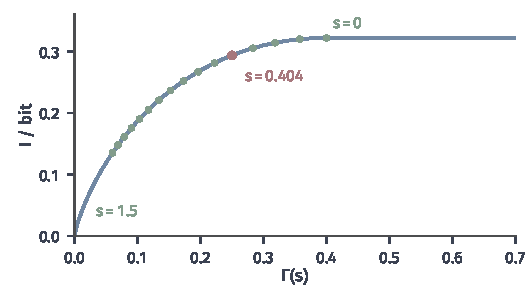
\includegraphics[width=90mm]{figures/07-probability/06-channel-coding/matplotlib/dcc-ba-cost/figure.pdf}
 \caption{Z信道、成本$c(0)=0$、$c(1)=1$时带乘子的Blahut–Arimoto迭代。蓝线为容量—成本函数的解析式，绿点为$s=0,0.1,\dots,1.5$各自迭代$400$轮得到的$(\Gamma(s),I)$，红点为二分求得的$s\approx0.404$，对应预算$\Gamma=0.25$。}
 \label{fig:dcc-ba-cost}
\end{BookInlineFigure}

带约束时，误差保证也要相应修改。上界来自弱对偶~\eqref{eq:dcc-weak-duality}：用定理~\ref{thm:dcc-kkt}中的恒等式，对任意$q$有
\[
 I(q)-s\sum_xq(x)c(x)\leq\max_x\bigl[D_{\mathrm{KL}}(W_x\Vert p_t)-s\,c(x)\bigr] ,
\]
所以
\[
 C(\Gamma)\leq\max_x\bigl[D_t(x)-s\,c(x)\bigr]+s\Gamma ,
\]
对任意$s\geq0$与任意一轮都成立。下界是当前输入的互信息$I(q_t)$，但只有在$\sum_xq_t(x)c(x)\leq\Gamma$时才算数：二分得到的$s$只使预算近似满足，若$q_t$略微超支，它的互信息不是$C(\Gamma)$的下界。所以报告结果时要同时核对实际的平均成本，必要时把$s$稍微调大，换取一个严格可行的输入。


\section{本章小结}
\label{sec:dcc-summary}

本章研究有限字母表上、编码器不使用反馈的离散无记忆信道。信道由转移矩阵$\bm{W}$给出，发送端能选择的是输入分布与码本；可靠传输的含义是码长增长时错误概率趋于零，速率按比特每次信道使用计量。

\paragraph{主要结论}
\begin{itemize}
 \item 容量公式：$C=\max_qI(q)$。$I(q)$是单纯形上的连续凹函数，最大值存在，最优输出分布唯一；最优输入由条件~\eqref{eq:dcc-kkt}刻画：被使用的输入的散度$D_{\mathrm{KL}}(W_x\Vert p^{*})$都等于$C$，未使用的不超过$C$。对任意输出分布$r$，$\max_xD_{\mathrm{KL}}(W_x\Vert r)$是容量的上界。

 \item 块的信息：无记忆与无反馈保证$I(X^n;Y^n)\leq nC$，独立使用最优输入达到等号。

 \item 编码定理：码率$R<C$时，随机码本加联合典型解码使平均错误趋于零，删去一半消息后最大错误也趋于零；码率$R>C$时，Fano不等式与数据处理给出$P_{\mathrm{e}}\geq1-C/R-1/(nR)$，错误不能趋于零。定理对$R=C$及有限块长不作承诺。

 \item 二元信道：二元对称信道$C=1-h_2(p)$，二元擦除信道$C=1-\varepsilon$；均匀输入最优来自交换对称性，Z信道的最优输入是$0.4$。已知错误位置的擦除比未知位置的翻转损失少，差值$h_2(p)-p$是定位错误的代价。

 \item 成本约束：逐条码字的预算下，容量是容量—成本函数$C(\Gamma)$，它单调、凹，切线斜率是预算的边际价值；可达性需要为预算留出余量，预算等于最小成本时改用受限字母表。

 \item 数值计算：Blahut–Arimoto迭代按$2^{D_{\mathrm{KL}}(W_x\Vert p_t)}$乘性地重新加权输入，每轮给出严格的上下界，下界误差不超过$D_{\mathrm{KL}}(q^{*}\Vert q_0)/(T+1)$；初始分布须有完整支撑，停止依据是上下界之差而不是迭代的变化量。
\end{itemize}

\paragraph{对比}
本章有几组容易混淆的概念，表~\ref{tab:dcc-summary-contrast}把它们并列。

\begin{BookInlineTable}
 \centering
 \caption{本章几组相邻概念的区别。}
 \label{tab:dcc-summary-contrast}
 \begin{tabular}{p{18mm}p{39mm}p{39mm}}
  \toprule
  对象 & 前者 & 后者 \\
  \midrule
  两个容量 & $C_{\mathrm{op}}$：可靠码率的上确界 & $C$：单次互信息的最大值 \\
  两种错误 & 平均错误：均匀消息下的错误率 & 最大错误：每条消息的保证 \\
  定理两向 & 可达性：存在好码，不给构造 & 逆定理：对一切码成立的限制 \\
  两种损坏 & 翻转：位置未知，$1-h_2(p)$ & 擦除：位置可见，$1-\varepsilon$ \\
  两种成本 & 期望成本：输入分布的约束 & 逐条预算：每条码字的约束 \\
  两种停止 & 迭代变化小：不是证书 & $U_t-L_t$小：严格的误差保证 \\
  \bottomrule
 \end{tabular}
\end{BookInlineTable}

容量回答“最多能多快”，没有回答“给定块长需要多少冗余”和“怎样以可承受的计算量编码与解码”。随机码本不可存储，典型性解码要搜索指数多个码字；有限长度的纠错构造与性能比较由第~\ref{chap:channel-codes}章展开。下一章先把输入字母从有限集合换成受功率限制的实数，研究高斯噪声下的容量，见第~\ref{chap:gaussian-channel-capacity}章。

